% ╔══════════════════════════════════════════════════════════════════════════════╗
% ║     PLANTILLA INSTITUCIONAL - INSTITUTO ATENEO DE COLIMA                      ║
% ║     Investigación Documental: Corrupción en México (2006-2012)                ║
% ║     Metodología: DIAC (Diseño Anidado Concurrente) - CUAL + cuan             ║
% ╚══════════════════════════════════════════════════════════════════════════════╝

\documentclass[12pt,letterpaper,oneside,openany]{book}

% ═══════════════════════════════════════════════════════════════════════════════
% CONFIGURACIÓN DE MÁRGENES Y GEOMETRÍA
% ═══════════════════════════════════════════════════════════════════════════════

\usepackage[margin=2.5cm,top=3.5cm,bottom=3.5cm,headheight=3cm,headsep=1.5cm]{geometry}

% ═══════════════════════════════════════════════════════════════════════════════
% ENCODING, IDIOMA Y TIPOGRAFÍA
% ═══════════════════════════════════════════════════════════════════════════════

\usepackage[utf8]{inputenc}
\usepackage[T1]{fontenc}
\usepackage[spanish,es-tabla,es-nodecimaldot]{babel}

% Tipografía profesional: Times New Roman para cuerpo, Helvetica para títulos
\usepackage{mathptmx}       % Times New Roman para el cuerpo
\usepackage{helvet}         % Helvetica para títulos
\renewcommand{\familydefault}{\sfdefault}  % Sans-serif por defecto para uniformidad institucional

% ═══════════════════════════════════════════════════════════════════════════════
% PAQUETES ESENCIALES
% ═══════════════════════════════════════════════════════════════════════════════

\usepackage{graphicx}
\usepackage{xcolor}
\usepackage{colortbl}
\usepackage{booktabs}
\usepackage{longtable}
\usepackage{array}
\usepackage{multirow}
\usepackage{float}
\usepackage{fancyhdr}
\usepackage{fancybox}
\usepackage{titlesec}
\usepackage{setspace}
\usepackage{pdflscape}
\usepackage{amssymb}
\usepackage{amsmath}
\usepackage{url}
\usepackage{watermark}                    % Marca de agua
\usepackage[authoryear,round]{natbib}     % Bibliografía APA
\usepackage[colorlinks=true,linkcolor=ateneo-blue!70!black,citecolor=ateneo-blue!70!black,urlcolor=ateneo-blue!70!black]{hyperref}

% ═══════════════════════════════════════════════════════════════════════════════
% COLORES INSTITUCIONALES - INSTITUTO ATENEO DE COLIMA
% ═══════════════════════════════════════════════════════════════════════════════

\definecolor{ateneo-purple}{HTML}{A6266C}  % Púrpura institucional (logo)
\definecolor{ateneo-blue}{HTML}{2E5090}    % Azul académico
\definecolor{ateneo-gray}{HTML}{4A4A4A}    % Gris corporativo
\definecolor{ateneo-light}{HTML}{F5F5F5}   % Fondo claro
\definecolor{documental}{HTML}{D35400}     % Naranja para identificación "ESTUDIO DOCUMENTAL"

% ═══════════════════════════════════════════════════════════════════════════════
% ESPACIADO Y FORMATO DE PÁRRAFOS
% ═══════════════════════════════════════════════════════════════════════════════

\setlength{\parindent}{0pt}
\setlength{\parskip}{0.72em}
\onehalfspacing

% ═══════════════════════════════════════════════════════════════════════════════
% FORMATO DE SECCIONES Y SUBSECCIONES
% ═══════════════════════════════════════════════════════════════════════════════

\titleformat{\chapter}[block]
  {\normalfont\sffamily\Large\bfseries\color{ateneo-purple}}
  {\thechapter.}{0.5em}{}

\titleformat{\section}[block]
  {\normalfont\sffamily\large\bfseries\color{ateneo-blue}}
  {\thesection.}{0.5em}{}[\titlerule]

\titleformat{\subsection}[block]
  {\normalfont\sffamily\normalsize\bfseries}
  {\thesubsection.}{0.5em}{}

\titleformat{\subsubsection}[runin]
  {\normalfont\sffamily\small\itshape}
  {\thesubsubsection.}{0.5em}{}

% ═══════════════════════════════════════════════════════════════════════════════
% ENCABEZADOS Y PIES DE PÁGINA (FANCYHDR)
% ═══════════════════════════════════════════════════════════════════════════════

\pagestyle{fancy}
\fancyhf{}
\fancyhead[L]{
\includegraphics[height=0.8cm]{img/image1.png}}
\fancyhead[C]{\small\textbf{Instituto Ateneo de Colima}\\Investigación Documental}
\fancyhead[R]{\textit{Corrupción 2006–2012}}
\fancyfoot[C]{\thepage}
\renewcommand{\headrulewidth}{0.4pt}
\renewcommand{\footrulewidth}{0.4pt}

% Estilos especiales para portada
\fancypagestyle{portada}{
  \fancyhf{}
  \renewcommand{\headrulewidth}{0pt}
  \renewcommand{\footrulewidth}{0pt}
}

% ═══════════════════════════════════════════════════════════════════════════════
% MARCA DE AGUA (WATERMARK) - "ESTUDIO DOCUMENTAL"
% ═══════════════════════════════════════════════════════════════════════════════

\ThisULCornerWallPaper{0.15}{img/image1.png}  % Logo en esquina superior derecha, 15% tamaño

% Marca de agua textual en primer plano
\usepackage{tikz}
\usetikzlibrary{shapes.misc}
\AddToShipoutPicture{
  \begin{tikzpicture}[remember picture, overlay]
    \node[
      text=documental!10,
      font=\fontsize{72}{72}\bfseries\sffamily,
      rotate=45,
      opacity=0.1
    ] at (current page.center) {DOCUMENTAL};
  \end{tikzpicture}
}

% ═══════════════════════════════════════════════════════════════════════════════
% COMANDO PERSONALIZADO PARA NOTA METODOLÓGICA
% ═══════════════════════════════════════════════════════════════════════════════

\newcommand{\nota}[1]{%
  \begin{center}
  \fcolorbox{ateneo-blue}{ateneo-light}{\parbox{0.9\textwidth}{\small\textbf{Nota metodológica:} #1}}
  \end{center}
}

\newcommand{\pendiente}[1]{\textcolor{red}{[\textbf{PENDIENTE:} #1]}}

\newcommand{\siglas}[1]{\textsc{#1}}

% ═══════════════════════════════════════════════════════════════════════════════
% BIBLIOGRAFÍA EN ESTILO APA 7
% ═══════════════════════════════════════════════════════════════════════════════

\bibliographystyle{apalike}
\setcitestyle{authoryear,round,citesep={;},aysep={,},yysep={,}}

% ═══════════════════════════════════════════════════════════════════════════════
% METADATOS DEL DOCUMENTO
% ═══════════════════════════════════════════════════════════════════════════════

\title{%
  {\Large\sffamily\bfseries INSTITUTO ATENEO DE COLIMA}\\[0.3cm]
  {\small INCORPORADO A LA UNIVERSIDAD DE COLIMA}\\[1.5cm]
  {\Huge\sffamily\bfseries Corrupción en México durante el sexenio de Felipe Calderón}\\
  {\LARGE\sffamily (2006–2012)}\\[0.5cm]
  {\large Análisis estructural, financiero y de derechos humanos}\\
  {\normalsize a partir de los casos Genaro García Luna, Refinería Bicentenario y Guardería ABC}
}

\author{%
  \textbf{Alumnos:}\\
  Ulysses Emiliano González de la Cruz\\
  Ian Alexander Miramonges Vázquez\\[1cm]
  \textbf{Maestra:}\\
  María Elena Luna Angulo\\[0.5cm]
  \textbf{Materia:}\\
  Metodología de la Investigación
}

\date{Noviembre de 2026}

% ═══════════════════════════════════════════════════════════════════════════════
% DOCUMENTO PRINCIPAL
% ═══════════════════════════════════════════════════════════════════════════════

\begin{document}

% ───────────────────────────────────────────────────────────────────────────────
% PORTADA INSTITUCIONAL
% ───────────────────────────────────────────────────────────────────────────────

\thispagestyle{portada}
\begin{center}
  \vspace*{1.5cm}
  
  % Logo institucional
  
\includegraphics[height=3cm]{img/image1.png}\\[1.5cm]
  
  {\Large\sffamily\bfseries INSTITUTO ATENEO DE COLIMA}\\[0.3cm]
  {\normalsize INCORPORADO A LA UNIVERSIDAD DE COLIMA}\\[2cm]
  
  % Línea decorativa
  {\color{ateneo-purple}\rule{0.8\textwidth}{2pt}}\\[0.8cm]
  
  {\Huge\sffamily\bfseries Corrupción en México durante el sexenio\\de Felipe Calderón (2006–2012)}\\[0.8cm]
  
  {\large\sffamily Análisis estructural, financiero y de derechos humanos\\
  a partir de los casos Genaro García Luna, Refinería Bicentenario y Guardería ABC}\\[0.8cm]
  
  % Línea decorativa
  {\color{ateneo-purple}\rule{0.6\textwidth}{1.5pt}}\\[2.5cm]
  
  % Información académica
  \begin{tabular}{rl}
    \textbf{Materia:} & METODOLOGÍA DE LA INVESTIGACIÓN \\[0.3cm]
    \textbf{Alumnos:} & Ulysses Emiliano González de la Cruz \\
                      & Ian Alexander Miramonges Vázquez \\[0.3cm]
    \textbf{Maestra:} & María Elena Luna Angulo \\[0.3cm]
    \textbf{Tipo de estudio:} & \textcolor{documental}{\textbf{INVESTIGACIÓN DOCUMENTAL}} \\
                              & \textit{Diseño Anidado Concurrente (DIAC: CUAL + cuan)} \\[0.3cm]
    \textbf{Fecha:} & Noviembre de 2026
  \end{tabular}
  
  \vfill
  
  {\small Colima, México}
  
\end{center}

\clearpage

% ───────────────────────────────────────────────────────────────────────────────
% NOTA METODOLÓGICA EN PORTADA INTERIOR
% ───────────────────────────────────────────────────────────────────────────────

\thispagestyle{fancy}

\begin{center}
  {\Large\sffamily\bfseries Declaración metodológica}
\end{center}

\vspace{1cm}

\nota{%
  Este documento constituye un \textbf{estudio documental} de casos múltiples 
  conforme a los estándares de Hernández Sampieri, Fernández Collado y Baptista 
  Lucio (2014). La investigación se estructuró bajo un \textbf{Diseño Anidado 
  Concurrente de Modelo Dominante (DIAC: CUAL + cuan)} que articula evidencia 
  cualitativa documental triangulada (resoluciones judiciales, auditorías oficiales 
  y doctrina académica) con indicadores cuantitativos secundarios descriptivos 
  (IPC 2025, ENCIG 2025, montos auditados). Los hallazgos ofrecen alcance 
  \textbf{analíticamente transferible} pero no estadísticamente generalizable 
  a la Administración Pública Federal 2006–2012.
}

\vspace{2cm}

\begin{center}
  {\sffamily\bfseries ÍNDICE DE CONTENIDOS}
\end{center}

\tableofcontents

\clearpage

% ───────────────────────────────────────────────────────────────────────────────
% LISTAS DE TABLAS Y FIGURAS
% ───────────────────────────────────────────────────────────────────────────────

\listoftables
\clearpage

\listoffigures
\clearpage

% ═══════════════════════════════════════════════════════════════════════════════
% CONTENIDO PRINCIPAL (CAPÍTULOS)
% ═══════════════════════════════════════════════════════════════════════════════

% Capítulo 1: Resumen y palabras clave
\chapter*{Resumen ejecutivo y palabras clave}
\addcontentsline{toc}{chapter}{Resumen ejecutivo y palabras clave}

En la presente investigación se analizaron los mecanismos causales y los efectos 
institucionales, financieros y en materia de derechos humanos derivados de la 
corrupción en México durante el sexenio de Felipe Calderón (2006–2012), con 
seguimiento judicial y fiscal hasta noviembre de 2026. El estudio se estructuró 
bajo un \textbf{Diseño Anidado Concurrente de Modelo Dominante (DIAC: CUAL + cuan)}, 
no experimental, retrospectivo y de estudio de casos múltiples.

La muestra no probabilística intencional comprendió tres casos principales 
---Genaro García Luna, Refinería Bicentenario y Guardería ABC---, complementados 
con dos casos de contraste contemporáneo (Veracruz y Refinería Olmeca/Dos Bocas) 
para examinar el encuadre mediático. La vertiente cualitativa trianguló resoluciones 
judiciales, auditorías de la Auditoría Superior de la Federación y doctrina académica 
mexicana e internacional, mientras que la vertiente cuantitativa anidada sistematizó 
indicadores descriptivos oficiales del IPC 2025, la ENCIG 2025 y pasivos auditados.

Los hallazgos documentaron captura institucional y desvío contractual en seguridad 
pública, endeudamiento y gasto improductivo sin candados transexenales en 
megainfraestructura, y dilución regulatoria con conflicto de interés y consecuencias 
letales en servicios subrogados. Se concluyó que los tres casos aportaron evidencia 
documental congruente con la hipótesis de trabajo, con alcance analíticamente 
transferible mas no estadísticamente generalizable a toda la Administración Pública Federal.

\vspace{1cm}

{\sffamily\bfseries Palabras clave:} Corrupción sistémica; captura del Estado; 
sexenio 2006–2012; rendición de cuentas; megainfraestructura; subrogación; 
derechos humanos; diseño mixto DIAC; encuadre mediático (framing).

\clearpage

% Capítulo 2: Introducción
\chapter{Introducción}

% ═══════════════════════════════════════════════════════════════════════════════
% INTRODUCCIÓN - INSTITUTO ATENEO DE COLIMA
% Estudio Documental: Corrupción en México (2006-2012)
% ═══════════════════════════════════════════════════════════════════════════════

\nota{
  Este capítulo introduce el problema de investigación desde una perspectiva 
  documental basada en evidencia oficial (ASF, SCJN, CNDH, CIDH, DOJ) y doctrina 
  académica arbitrada (Casar y Cejudo 2024; Merino 2024; Sandoval Ballesteros 2024).
}

\section{Contexto y perspectiva}

Con frecuencia, la historia de la corrupción en México suele narrarse al revés: la atención pública se concentra en el escándalo pasajero, la consigna viral o el enfrentamiento partidista, mientras rara vez se analiza con la cabeza fría el proceso institucional que permitió llegar a ese desenlace y el costo humano que recayó sobre la población. Así como detrás de los resultados visibles existen siempre planes, omisiones o rutinas acumuladas, el propósito de este reporte no consistió en repartir culpas por simpatía política ni en reproducir el ruido mediático, sino en examinar ---mediante evidencia oficial, auditorías y resoluciones judiciales--- qué falló estructuralmente en tres episodios decisivos y de qué manera sus secuelas comprometen lo más valioso para una sociedad: la vida, la salud, la seguridad y el patrimonio colectivo.

Desde la perspectiva científica, la corrupción constituye un fenómeno multidimensional que trasciende el plano estrictamente moral o penal para consolidarse como un problema estructural con repercusiones directas sobre el erario, la calidad de los servicios públicos, la vigencia de los derechos humanos y la legitimidad democrática \citep{inegi2016,monsivais2020,reyesheroles2003}. Su persistencia a través de distintas administraciones revela la consolidación de una corrupción sistémica y estructural, en la que las reglas formales son capturadas por redes de poder lícitas e ilícitas y la impunidad se institucionaliza \citep{casar2024,merino2024,sandoval2024}.

En este estudio se delimitó como periodo nuclear el sexenio de Felipe Calderón Hinojosa (2006--2012), administración que concluyó con una calificación de 34 sobre 100 puntos para México en el Índice de Percepción de la Corrupción (IPC) de Transparencia Internacional (2026). Durante esa etapa se gestaron expedientes de alto impacto cuyas consecuencias jurídicas, financieras y sociales se extendieron hasta noviembre de 2026, según se documentó en informes de la Auditoría Superior de la Federación (\siglas{asf}), sentencias de la Suprema Corte de Justicia de la Nación (\siglas{scjn}), recomendaciones de la Comisión Nacional de los Derechos Humanos (\siglas{cndh}), informes de la Comisión Interamericana de Derechos Humanos (\siglas{cidh}) y procesos penales y civiles sustanciados en tribunales de Estados Unidos \citep{asf2013,asf2015,asf2016,cidh2020,cndh2009,doj2024,scjn2010,scjn2025,uif2025,uif2026}.

La investigación examinó tres casos principales representativos de mecanismos diferenciados: la captura del aparato de seguridad pública y el desvío contractual en el caso de Genaro García Luna; las deficiencias de preinversión y los pasivos transexenales en la Refinería Bicentenario en Tula, Hidalgo; y la subrogación desregulada con conflicto de interés en la Guardería ABC. De manera complementaria, se incorporaron dos casos de contraste contemporáneo (el saqueo hospitalario en Veracruz y la Refinería Olmeca en Dos Bocas) con el fin exclusivo de contrastar el impacto verificable sobre las víctimas frente al sesgo del encuadre mediático (framing). El informe se organizó conforme a los estándares metodológicos de Hernández Sampieri, Fernández Collado y Baptista Lucio (2014), integrando justificación, planteamiento, marco teórico fortalecido con doctrina mexicana, diseño mixto DIAC, análisis de casos, discusión de rigor y limitaciones, conclusiones, referencias y apéndices instrumentales.

\section{Objetivos del estudio}

Este estudio documental se propuso tres objetivos centrales:

\begin{itemize}
  \item Analizar los mecanismos causales y los efectos estructurales ---institucionales, financieros y en materia de derechos humanos--- de la corrupción en México durante el sexenio 2006--2012 mediante un diseño mixto de modelo dominante cualitativo (DIAC: CUAL + cuan).
  
  \item Documentar, mediante evidencia oficial verificable, cómo decisiones administrativas adoptadas hace más de una década continuaron generando pasivos fiscales, litigios y demandas de justicia vigentes en 2026.
  
  \item Contrastar el daño real acreditado en auditorías y resoluciones judiciales con las narrativas mediáticas (framing) que suelen simplificar fenómenos complejos en consignas virales.
\end{itemize}

% FIGURA PENDIENTE
\begin{figure}[H]
\centering
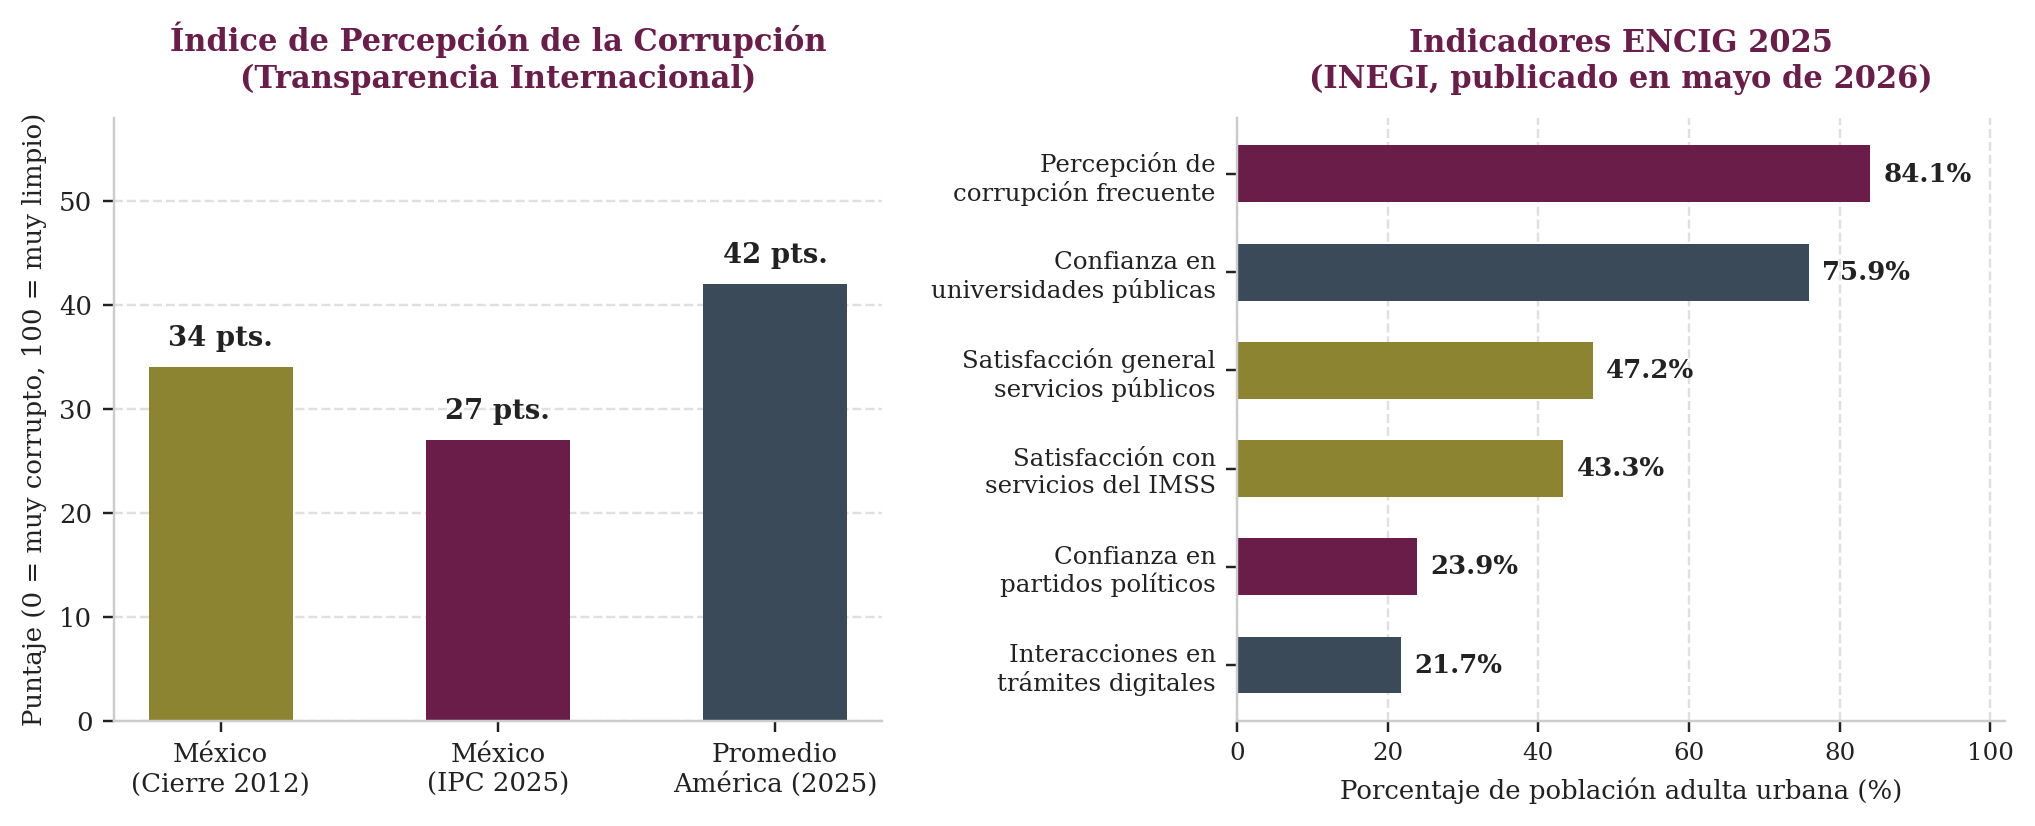
\includegraphics[width=0.9\textwidth]{img/image3.png} % Figura 1: Evolución IPC 2012 vs 2025 + ENCIG 2025
\caption{Evolución del Índice de Percepción de la Corrupción (2012 vs. 2025) e indicadores nacionales de la ENCIG 2025. Fuente: Elaboración propia con datos de Transparencia Internacional (2026) e INEGI (2026).}
\label{fig:ipc-encig}
\end{figure}

\clearpage

% Capítulo 3: Justificación
\chapter{Justificación de la investigación}

% ═══════════════════════════════════════════════════════════════════════════════
% JUSTIFICACIÓN - INSTITUTO ATENEO DE COLIMA
% Estudio Documental: Corrupción en México (2006-2012)
% ═══════════════════════════════════════════════════════════════════════════════

\nota{
  Esta sección articula cinco dimensiones de justificación metodológica: social, 
  académica, práctica, utilidad metodológica y viabilidad, todas fundamentadas en 
  fuentes oficiales verificables y doctrina académica arbitrada.
}

\section{Relevancia social}

La literatura internacional en derechos humanos establece que la corrupción no es un delito sin víctimas, sino una práctica que vulnera directa o indirectamente derechos económicos, sociales y culturales ---entre ellos la vida, la salud, la seguridad y el acceso equitativo a bienes públicos---, afectando de forma desproporcionada a los sectores vulnerables y profundizando la desigualdad estructural \citep{cidh2019,cndh2019,rios2021}. 

En México, el fenómeno opera como un impuesto regresivo de alcance cotidiano: de acuerdo con la Encuesta Nacional de Calidad e Impacto Gubernamental (ENCIG) 2025 del INEGI, publicada en mayo de 2026, 84.1\,\% de la población adulta urbana percibió que los actos de corrupción gubernamental son frecuentes o muy frecuentes, mientras que los pagos indebidos en trámites extrajeron 17,707.4 millones de pesos anuales ---3,865 pesos promedio por víctima---, el costo real más alto de la última década \citep{inegi2026,imco2026}. El análisis retrospectivo de los expedientes clave del periodo 2006--2012 permitió evidenciar cómo decisiones administrativas adoptadas hace más de una década continuaron generando pasivos fiscales, litigios y demandas de justicia vigentes en 2026.

\section{Relevancia académica}

El estudio científico de la corrupción mexicana demanda articular marcos conceptuales internacionales con la tradición académica nacional en ciencia política, sociología, antropología, economía política y derecho público. En esta investigación se integraron aportes clásicos e internacionales ---Nye (1967), Rose-Ackerman (1999, 2004), Garay Salamanca y Salcedo-Albarán (2012), Cancino y el BID (2020), Dávid-Barrett y Fazekas (2020) y Rezzoagli et al. (2021)--- con obras medulares de investigadores mexicanos como Casar y Cejudo (2024), Merino (2024), López Ayllón y Merino (2009), Peschard (2017), Arellano Gault (2012, 2020), Lomnitz (2000), Zaid (2019), Sandoval Ballesteros (2009, 2024), Serna de la Garza (2010), Vázquez Valencia (2019), Astorga (2007, 2015), Flores Pérez (2009) y Reyes Heroles (2003). Dicha articulación permitió contrastar marcos teóricos complejos con resoluciones judiciales y auditorías oficiales verificables.

\section{Relevancia práctica}

Diversos diagnósticos institucionales coinciden en que el principal obstáculo para contener la corrupción en México no radica en la ausencia de legislación, sino en la brecha de implementación entre la norma jurídica y su cumplimiento efectivo \citep{casar2024,lopezayllon2009,peschard2017}. Al reconstruir los factores que hicieron posibles la concentración discrecional del mando policial, la contratación de megainfraestructura sin candados transexenales y la expansión de guarderías subrogadas sin vigilancia independiente, los hallazgos de este trabajo ofrecieron insumos concretos para el diseño de políticas de fiscalización autónoma, digitalización de trámites y control regulatorio sobre servicios concesionados.

\section{Utilidad metodológica}

Desde el punto de vista metodológico, el estudio aportó un procedimiento replicable para investigar fenómenos de gran corrupción mediante un Diseño Anidado Concurrente de Modelo Dominante (DIAC: CUAL + cuan) aplicado a estudios de casos múltiples \citep{hernandez2014}. En lugar de analizar por separado las resoluciones judiciales, las auditorías financieras o el discurso periodístico, se diseñaron y aplicaron dos instrumentos documentales estructurados ---una Ficha de Registro Jurídico-Institucional y Hemerográfico (Apéndice A) y una Matriz Comparativa de Variables, Dimensiones e Indicadores por Caso (Apéndice B)--- que permitieron triangular evidencia probatoria oficial con estadísticas descriptivas secundarias y análisis de encuadre mediático (framing), generando metainferencias trazables.

\section{Viabilidad del estudio}

La investigación resultó plenamente viable desde las dimensiones documental, técnica, temporal y financiera. Se dispuso de acceso abierto a fuentes primarias oficiales y de alta confiabilidad ---informes de la ASF, engroses y dictámenes de la SCJN, recomendaciones de la CNDH, informes de la CIDH, comunicados de la Unidad de Inteligencia Financiera (UIF), expedientes del Departamento de Justicia de Estados Unidos (DOJ), bases estadísticas del INEGI y reportes de Transparencia Internacional---, complementadas con libros y artículos científicos dictaminados. La selección acotada de tres casos principales y dos de contraste contemporáneo garantizó profundidad analítica sin requerir financiamiento externo ni trabajo de campo en entornos de riesgo.

\clearpage

% Capítulo 4: Planteamiento
\chapter{Planteamiento del problema}

% ═══════════════════════════════════════════════════════════════════════════════
% PLANTEAMIENTO DEL PROBLEMA - INSTITUTO ATENEO DE COLIMA
% Estudio Documental: Corrupción en México (2006-2012)
% ═══════════════════════════════════════════════════════════════════════════════

\nota{
  Este capítulo plantea el problema de investigación desde una perspectiva 
  documental basada en evidencia oficial (ASF, SCJN, CNDH, CIDH, DOJ) y 
  doctrina académica (Casar y Cejudo 2024; Merino 2024). Se enfatiza la 
  brecha entre normatividad anticorrupción y aplicación efectiva.
}

\section{Contexto institucional y normativo}

A pesar de contar con una extensa arquitectura constitucional, administrativa y penal ---integrada por el artículo 113 constitucional, el Sistema Nacional Anticorrupción (SNA), la Ley General de Responsabilidades Administrativas (LGRA), el Título Décimo del Código Penal Federal y convenciones vinculantes ante la ONU, la OEA y la OCDE---, México se mantuvo en niveles críticos de corrupción percibida y experimentada \citep{cpeum,lgra,casar2024,merino2024}. En el IPC 2025, difundido en febrero de 2026 por Transparencia Internacional, el país obtuvo 27 de 100 puntos y ocupó el lugar 141 de 182 naciones evaluadas, último puesto entre los países miembros de la OCDE y siete puntos por debajo de la calificación de 34 puntos registrada al concluir 2012 \citep{transparencia2026,mcci2026b}.

Durante el sexenio de Felipe Calderón Hinojosa (2006--2012), la fragilidad de los contrapesos horizontales y verticales favoreció el desarrollo de esquemas de corrupción de alto calado cuyos efectos rebasaron los límites del periodo presidencial \citep{astorga2015,lopezayllon2009}. En primer lugar, la concentración de mando, presupuesto e inteligencia en la Secretaría de Seguridad Pública (SSP) permitió la colusión de su titular, Genaro García Luna, con el Cártel de Sinaloa y la operación de una red de desvío de recursos mediante contratos tecnológicos y empresas offshore \citep{doj2024garcialuna,uif2025,uif2026}. En segundo término, proyectos estratégicos impulsados sin candados técnicos vinculantes, como la Refinería Bicentenario en Tula, comprometieron endeudamiento subnacional y miles de millones de pesos federales sin concluir una infraestructura productiva \citep{asf2015,asf2016}. En tercer lugar, la expansión acelerada de guarderías subrogadas del IMSS bajo estándares flexibilizados, ausencia de inspección eficaz y conflictos de interés culminó en el incendio de la Guardería ABC, con un saldo de 49 niñas y niños fallecidos \citep{cndh2009,scjn2010}.

A estos problemas estructurales se sumó una distorsión persistente en el espacio público: los encuadres mediáticos (framing) y la polarización partidista suelen simplificar fenómenos complejos en símbolos virales, mezclando delitos acreditados, negligencia regulatoria, ineficiencia administrativa y afirmaciones sin sustento sanitario o financiero \citep{solamorales2019}. Ante este escenario, resultó necesario examinar de manera sistemática y verificable cómo se configuraron los mecanismos de corrupción en los tres casos del periodo 2006--2012 y cuál fue su impacto real sobre las instituciones, el erario y los derechos humanos.

\section{Evaluación de las deficiencias en el conocimiento del problema}

Conforme a los criterios de planteamiento establecidos por Hernández Sampieri et al. (2014), la revisión inicial de la literatura evidenció una brecha relevante en el conocimiento acumulado sobre la corrupción del sexenio 2006--2012. Por un lado, existen expedientes jurídicos y resoluciones judiciales especializadas (como las sentencias penales y civiles estadounidenses contra García Luna o los fallos de la SCJN y la CIDH sobre Guardería ABC); por otro, auditorías técnicas y financieras de la ASF sobre obra pública y pasivos estatales; y, en una vertiente separada, estudios de comunicación política acerca del encuadre mediático (framing) de los escándalos públicos. Sin embargo, se identificó una escasez de estudios integradores que articulen simultáneamente esas tres dimensiones ---evidencia jurídico-judicial, impacto financiero auditado y análisis de encuadre mediático--- incorporando las resoluciones emitidas entre 2024 y noviembre de 2026. Esta investigación se propuso cubrir dicha deficiencia mediante un análisis comparado de casos múltiples.

\section{Consecuencias éticas de la investigación}

De acuerdo con Hernández Sampieri et al. (2014), todo planteamiento científico exige evaluar las consecuencias éticas derivadas de su ejecución y difusión. Dado que el estudio abordó delitos graves, procesos judiciales activos y una tragedia que involucró a menores de edad (Guardería ABC), se aplicaron tres principios éticos estrictos: primero, el uso exclusivo de fuentes públicas, oficiales y verificables (resoluciones judiciales, auditorías, recomendaciones de derechos humanos y literatura académica), evitando especulaciones o señalamientos carentes de soporte documental; segundo, el respeto irrestricto a la dignidad de las víctimas y sus familias, excluyendo descripciones sensacionalistas o cualquier forma de revictimización; y tercero, el mantenimiento de un balance probatorio objetivo que registró explícitamente las posturas de descargo de los actores públicos señalados y la continuidad transexenal de diversos entramados, evitando sesgos partidistas.

\clearpage

% Capítulo 5: Preguntas y objetivos
\chapter{Preguntas de investigación y objetivos}

% ═══════════════════════════════════════════════════════════════════════════════
% PREGUNTAS Y OBJETIVOS - INSTITUTO ATENEO DE COLIMA
% Estudio Documental: Corrupción en México (2006-2012)
% ═══════════════════════════════════════════════════════════════════════════════

\nota{
  Este capítulo presenta la pregunta central y los objetivos de investigación 
  formulados conforme a los estándares de Hernández Sampieri (2014) para 
  estudios documentales de casos múltiples. La pregunta central guía el análisis 
  documental de los tres casos principales.
}

\section{Preguntas de investigación}

\subsection{Pregunta central}

¿De qué manera los esquemas de corrupción gestados durante el sexenio de Felipe Calderón (2006--2012) impactaron la integridad institucional, las finanzas públicas y los derechos humanos en México, a partir de los casos de Genaro García Luna, la Refinería Bicentenario y la Guardería ABC?

\subsection{Preguntas específicas}

\begin{enumerate}
  \item ¿De qué manera las distintas tipologías de corrupción ---desde prácticas incidentales hasta esquemas sistémicos y de captura estatal--- incidieron de forma verificable sobre el erario público, la legitimidad institucional y el ejercicio de los derechos humanos en México?
  
  \item ¿Cuál fue el nivel y la evolución empírica de la corrupción en México desde el cierre del sexenio 2006--2012 hasta las mediciones nacionales e internacionales más recientes (IPC 2025 y ENCIG 2025)?
  
  \item ¿Qué condiciones institucionales y mecanismos estructurales posibilitaron la captura del aparato de seguridad en el caso Genaro García Luna, los pasivos financieros en la Refinería Bicentenario y el desorden regulatorio con conflicto de interés en la Guardería ABC?
  
  \item ¿En qué medida difiere la magnitud verificable del daño ocasionado a la población y a sus derechos humanos respecto del tratamiento que reciben determinados escándalos bajo el encuadre mediático (framing), al contrastar los casos del periodo 2006--2012 con episodios contemporáneos como Veracruz y Dos Bocas?
  
  \item ¿Qué controles institucionales, mecanismos de rendición de cuentas y rediseños de incentivos sugiere la evidencia documental y teórica para reducir la brecha entre la normatividad anticorrupción y su aplicación efectiva en México?
\end{enumerate}

\section{Objetivos}

\subsection{Objetivo General}

Analizar los mecanismos causales y los efectos estructurales ---institucionales, financieros y en materia de derechos humanos--- de la corrupción en México durante el sexenio de Felipe Calderón (2006--2012), mediante un estudio documental de casos múltiples centrado en Genaro García Luna, la Refinería Bicentenario y la Guardería ABC, contrastando su impacto verificable con el tratamiento mediático del fenómeno.

\subsection{Objetivos Específicos}

\begin{enumerate}
  \item Sistematizar los fundamentos conceptuales y teóricos sobre la corrupción, sus tipologías jurídicas y sus efectos verificables sobre el erario, la legitimidad democrática y los derechos humanos, integrando doctrina internacional y mexicana.
  
  \item Describir el nivel, el costo económico y la trayectoria empírica de la corrupción en México a partir de indicadores secundarios oficiales de percepción agregada (IPC) y victimización directa (ENCIG), situando el cierre de 2012 en perspectiva longitudinal hasta 2026.
  
  \item Examinar el origen, los mecanismos de operación, las fallas de control y las resoluciones judiciales o de fiscalización de los tres casos emblemáticos del periodo 2006--2012 (Genaro García Luna, Refinería Bicentenario y Guardería ABC), junto con expedientes comparables del mismo sexenio.
  
  \item Contrastar el alcance real de las afectaciones a derechos humanos frente a la distorsión producida por el encuadre mediático (framing) mediante dos casos de contraste contemporáneo (Veracruz y Dos Bocas), derivando metainferencias sobre el fortalecimiento de la rendición de cuentas.
\end{enumerate}

\clearpage

% Capítulo 6: Marco teórico
\chapter{Marco teórico}

% ═══════════════════════════════════════════════════════════════════════════════
% MARCO TEÓRICO - INSTITUTO ATENEO DE COLIMA
% Estudio Documental: Corrupción en México (2006-2012)
% ═══════════════════════════════════════════════════════════════════════════════

\nota{
  Este capítulo desarrolla el marco teórico-conceptual articulando doctrina 
  internacional (Nye, Rose-Ackerman, Klitgaard) con tradición académica mexicana 
  (Casar y Cejudo, Merino, Sandoval Ballesteros). La base conceptual sustenta el 
  análisis documental de los tres casos principales.
}

\section{Fundamentación teórica (autores y contribuciones)}

En las ciencias sociales y jurídicas no existe una definición única de corrupción, pero sí un consenso operativo que la conceptualiza como la desviación de deberes públicos o fiduciarios orientada a obtener beneficios indebidos en perjuicio del interés general \citep{inegi2016}. Con el propósito de sustentar rigurosamente el análisis de los casos seleccionados y elevar la densidad de la literatura científica arbitrada, la fundamentación teórica se articuló en seis ejes que vinculan teoría internacional con el pensamiento académico mexicano:

\begin{enumerate}
  \item \textbf{Fundamentos político-institucionales, económicos y tipificación internacional:} Desde la ciencia política, Joseph S. Nye (1967) define la corrupción como la conducta que se aparta de los deberes formales de un cargo público por consideraciones pecuniarias o de estatus privado ---personal, familiar o grupal---, o que infringe normas contra formas indebidas de influencia privada. En el plano económico-relacional, Susan Rose-Ackerman (1999, 2004) plantea el mal uso del poder público para beneficio privado o político como un fenómeno bilateral que germina en la interfaz entre el Estado (regulador o contratante) y el sector privado, actuando como un impuesto regresivo que encarece servicios, distorsiona licitaciones y frena la inversión productiva. A nivel normativo internacional, Transparencia Internacional adopta la noción ampliada de abuso de poder encomendado para beneficio propio, mientras que la Convención de las Naciones Unidas contra la Corrupción (CNUCC) tipifica el soborno (arts. 15, 16 y 21), el peculado (arts. 17 y 22), el tráfico de influencias (art. 18) y el abuso de funciones (art. 19) \citep{unodc2003}.

  \item \textbf{Corrupción sistémica, Estado capturado y rendición de cuentas en México:} La Oficina de las Naciones Unidas contra la Droga y el Delito (UNODC, s. f.) y María Amparo Casar y Guillermo M. Cejudo (2024) distinguen entre corrupción incidental ---actos aislados controlables por el sistema--- y corrupción sistémica, en la cual las transgresiones se normalizan y prevalece la impunidad. En la doctrina política mexicana, Mauricio Merino (2024) profundiza este diagnóstico bajo la categoría de Estado capturado, sosteniendo que la corrupción permeó el aparato público al punto de operar como regla que captura cargos, presupuestos y decisiones administrativas. Previamente, Sergio López Ayllón y Mauricio Merino (2009) demostraron que la rendición de cuentas no constituye un simple trámite contable, sino un sistema integral que requiere contrapesos horizontales entre poderes, vigilancia vertical ciudadana y capacidad efectiva de sanción. En consonancia, Jacqueline Peschard (2017) advierte que el acceso a la información y la transparencia resultan condiciones necesarias pero insuficientes para contener la corrupción cuando carecen de fiscalización autónoma y consecuencias jurídicas vinculantes.

  \item \textbf{Raíces organizacionales, históricas y concentración del poder:} Para explicar por qué la corrupción persiste pese a reformas legales sucesivas, la literatura mexicana aporta explicaciones organizacionales, históricas y culturales. Desde la teoría de las organizaciones, David Arellano Gault (2012, 2020) concibe la corrupción como una relación social densa ---expresada en redes informales de favores y lealtades--- incrustada en rutinas burocráticas, por lo cual las respuestas meramente punitivas o voluntaristas fracasan si no rediseñan incentivos y procesos administrativos. Desde la antropología histórica, Claudio Lomnitz (2000) muestra cómo en México se configuró una frontera porosa entre lo público y lo privado en la que lealtades familiares y clientelares compiten con la legalidad formal, sustentando las categorías de nepotismo y conflicto de interés. A su vez, Gabriel Zaid (2019) identifica la raíz del problema en la concentración discrecional del poder y en lo que denomina «la propiedad privada de las funciones públicas», insistiendo en cuantificar sus efectos con datos verificables.

  \item \textbf{Corrupción estructural, megainfraestructura, desigualdad y subrogación:} En la vertiente de economía política y contratación estatal, Irma Eréndira Sandoval Ballesteros (2009, 2024) formula la teoría de la corrupción estructural y el doble fraude, argumentando que los procesos de privatización, concesión y contratación pública sin controles efectivos permiten que élites políticas y económicas capturen las reglas institucionales con daños patrimoniales sistémicos. Complementariamente, Viridiana Ríos (2021) demuestra mediante evidencia cuantitativa que las reglas capturadas y la opacidad institucional amplifican la desigualdad económica al castigar desproporcionadamente a los hogares de menores ingresos. En materia de grandes obras, Cancino y el Banco Interamericano de Desarrollo (BID, 2020) ---retomando a Bent Flyvbjerg--- documentan patrones de fracaso en megainfraestructura asociados a decisiones políticas prematuras, subestimación de costos y opacidad en preinversión, mientras que Dávid-Barrett y Fazekas (2020) evidencian cómo la discrecionalidad contractual y la falta de candados transexenales exponen los proyectos estratégicos al favoritismo partidista. En el ámbito de servicios delegados, Bruno Rezzoagli et al. (2021) y el jurista mexicano José María Serna de la Garza (2010) acreditan que la subrogación y privatización sin capacidad regulatoria independiente diluyen la responsabilidad administrativa del Estado y multiplican el conflicto de interés.

  \item \textbf{Macrocriminalidad, seguridad pública y captura institucional en 2006--2012:} El análisis del aparato de seguridad durante 2006--2012 encuentra sustento directo en la teoría de la captura del Estado y la macrocriminalidad. Luis Daniel Vázquez Valencia (2019) explica cómo estructuras ilícitas coactúan con gobiernos formalmente constitucionales para vaciar instituciones democráticas y vulnerar derechos humanos, mientras que Luis Jorge Garay Salamanca y Eduardo Salcedo-Albarán (2012) diferencian entre Captura del Estado (CAE) y Reconfiguración Cooptada del Estado (RCDE). En la sociología política mexicana, Luis Astorga (2007, 2015) analiza la relación histórica entre poder político, cuerpos de seguridad y narcotráfico, dedicando un examen específico a las fallas institucionales y la concentración de mando durante la presidencia de Felipe Calderón. Asimismo, Carlos Antonio Flores Pérez (2009) demuestra cómo la alternancia política sin una reforma policial integral ni controles efectivos posibilitó la penetración del crimen organizado en estructuras gubernamentales. Como respaldo documental de caso, la investigación periodística en formato libro de Diego Enrique Osorno (2010) complementa los expedientes jurídicos sobre las redes políticas y omisiones de supervisión en la tragedia de la Guardería ABC.

  \item \textbf{Derechos humanos, medición empírica, legitimidad y encuadre mediático:} Finalmente, la Comisión Interamericana de Derechos Humanos (CIDH, 2019), la CNDH (2019) y Anne Peters (en IIJ-UNAM, 2018) establecen que la corrupción vulnera derechos fundamentales y debe evaluarse por la magnitud del daño infligido a las víctimas. En México, Federico Reyes Heroles (2003) marcó el tránsito analítico de concebir la corrupción como un asunto moral («de los ángeles») a medirla objetivamente mediante indicadores y costos verificables («a los índices»). En la misma línea, Alejandro Monsiváis-Carrillo (2020) demuestra que la impunidad sostenida erosiona la legitimidad democrática, y Sola-Morales y Zurbano-Berenguer (2019) explican cómo el encuadre mediático (framing) y la espectacularización política distorsionan la jerarquía de los problemas públicos. En cuanto al horizonte preventivo, autores como Klitgaard (1988), Mungiu-Pippidi (2015) y la OCDE (2017) coinciden en que contener la corrupción exige reducir monopolios discrecionales, fortalecer contrapesos y consolidar sistemas de integridad pública.
\end{enumerate}

\section{Marco contextual: definiciones operativas y diagnóstico empírico}

\subsection{Definición de palabras clave}

Con el propósito de preservar rigor terminológico y distinguir entre delitos acreditados, faltas administrativas graves e ineficiencia gubernamental, en el reporte se emplearon las siguientes definiciones operativas:

\begin{table}[H]
\centering
\caption{Definición operativa de palabras clave de la investigación}
\label{tab:definiciones}
\small
\begin{tabular}{@{}p{3.5cm}p{10cm}@{}}
\toprule
\textbf{Concepto clave} & \textbf{Definición operativa} \\
\midrule
Corrupción & Abuso de un poder o cargo encomendado ---público o privado--- para obtener un beneficio indebido en perjuicio del interés general y las normas establecidas; articula abuso de poder, beneficio indebido y quiebre de la integridad \citep{transparencia2026,inegi2016}. \\
\addlinespace
Soborno o cohecho & Ofrecer, dar, solicitar o aceptar dinero, bienes o favores para que una autoridad ejecute u omita actos propios de sus funciones \citep{unodc2003}. \\
\addlinespace
Peculado o desvío de recursos & Apropiación o uso de fondos, bienes o recursos públicos para fines privados o distintos a los autorizados presupuestalmente. \\
\addlinespace
Tráfico de influencias & Utilización del cargo público o de relaciones con otros servidores públicos para inclinar decisiones administrativas, contrataciones o resoluciones en favor de terceros. \\
\addlinespace
Conflicto de interés & Situación en la que el juicio o desempeño imparcial de un servidor público se ve comprometido por intereses personales, familiares o de negocios \citep{lomnitz2000}. \\
\addlinespace
Captura del Estado & Proceso mediante el cual redes lícitas o criminales infiltran, cooptan y subordinan instituciones estatales clave para operar bajo amparo institucional e impunidad \citep{merino2024,vazquezvalencia2019}. \\
\addlinespace
Subrogación de servicios públicos & Delegación de la prestación de un servicio público estatal (como las estancias infantiles del IMSS) a operadores privados mediante concesiones sujetas a regulación y vigilancia del Estado \citep{leal2010,sernadelagarza2010}. \\
\addlinespace
Encuadre mediático (framing) & Selección y énfasis de determinados atributos o símbolos de un hecho público en medios y redes sociales, capaz de moldear la percepción social de causalidad y urgencia \citep{solamorales2019}. \\
\bottomrule
\end{tabular}
\end{table}

\subsection{Antecedentes de la investigación: panorama empírico y arquitectura jurídica}

La medición contemporánea de la corrupción en México combina índices internacionales de percepción agregada con encuestas nacionales de experiencia directa en trámites públicos \citep{reyesheroles2003,zaid2019}. En la Tabla~\ref{tab:indicadores} se sintetizaron los indicadores secundarios oficiales más recientes y su contraste longitudinal con el cierre del sexenio 2006--2012:

\begin{table}[H]
\centering
\caption{Indicadores oficiales de percepción, prevalencia y costo de la corrupción en México (2012--2026)}
\label{tab:indicadores}
\small
\begin{tabular}{@{}p{2.8cm}p{2.5cm}p{3.5cm}p{4cm}@{}}
\toprule
\textbf{Indicador} & \textbf{Fuente / Edición} & \textbf{Resultado en México} & \textbf{Contexto y relación longitudinal (2012--2026)} \\
\midrule
Índice de Percepción de la Corrupción (IPC) & Transparencia Internacional (IPC 2025, publ. feb. 2026) & 27 / 100 puntos (Posición 141 de 182 países) & Descenso de siete puntos respecto a los 34 puntos del cierre de 2012; último lugar de la OCDE y por debajo del promedio de América (42 pts.). \\
\addlinespace
Percepción de frecuencia & INEGI --- ENCIG 2025 (publ. mayo 2026) & 84.1\,\% de la población adulta urbana & Percibió actos de corrupción gubernamental como frecuentes o muy frecuentes; brechas estatales de 89\,\% (Michoacán, BC, CDMX) a 67\,\% (Querétaro). \\
\addlinespace
Prevalencia en trámites y servicios & INEGI --- ENCIG 2025 & 15.6\,\% (15,642 actos por cada 100 mil hab.) & Proporción de usuarios que enfrentaron al menos un acto de corrupción al gestionar trámites; únicamente 21.7\,\% de las interacciones fueron digitales. \\
\addlinespace
Costo económico directo & INEGI --- ENCIG 2025 & \$17,707.4 millones de pesos anuales & Equivalente a \$3,865 pesos promedio por víctima; representó el costo real más elevado en la última década \citep{imco2026}. \\
\addlinespace
Satisfacción y confianza institucional & INEGI --- ENCIG 2025 & 47.2\,\% satisfacción en servicios; 23.9\,\% confianza en partidos & Disminución frente al 50.0\,\% de 2023; el transporte público (36.9\,\%) y el IMSS (43.3\,\%) obtuvieron las menores evaluaciones, frente a 75.9\,\% de confianza en universidades públicas. \\
\bottomrule
\end{tabular}
\end{table}

% FIGURA PENDIENTE
\begin{figure}[H]
\centering
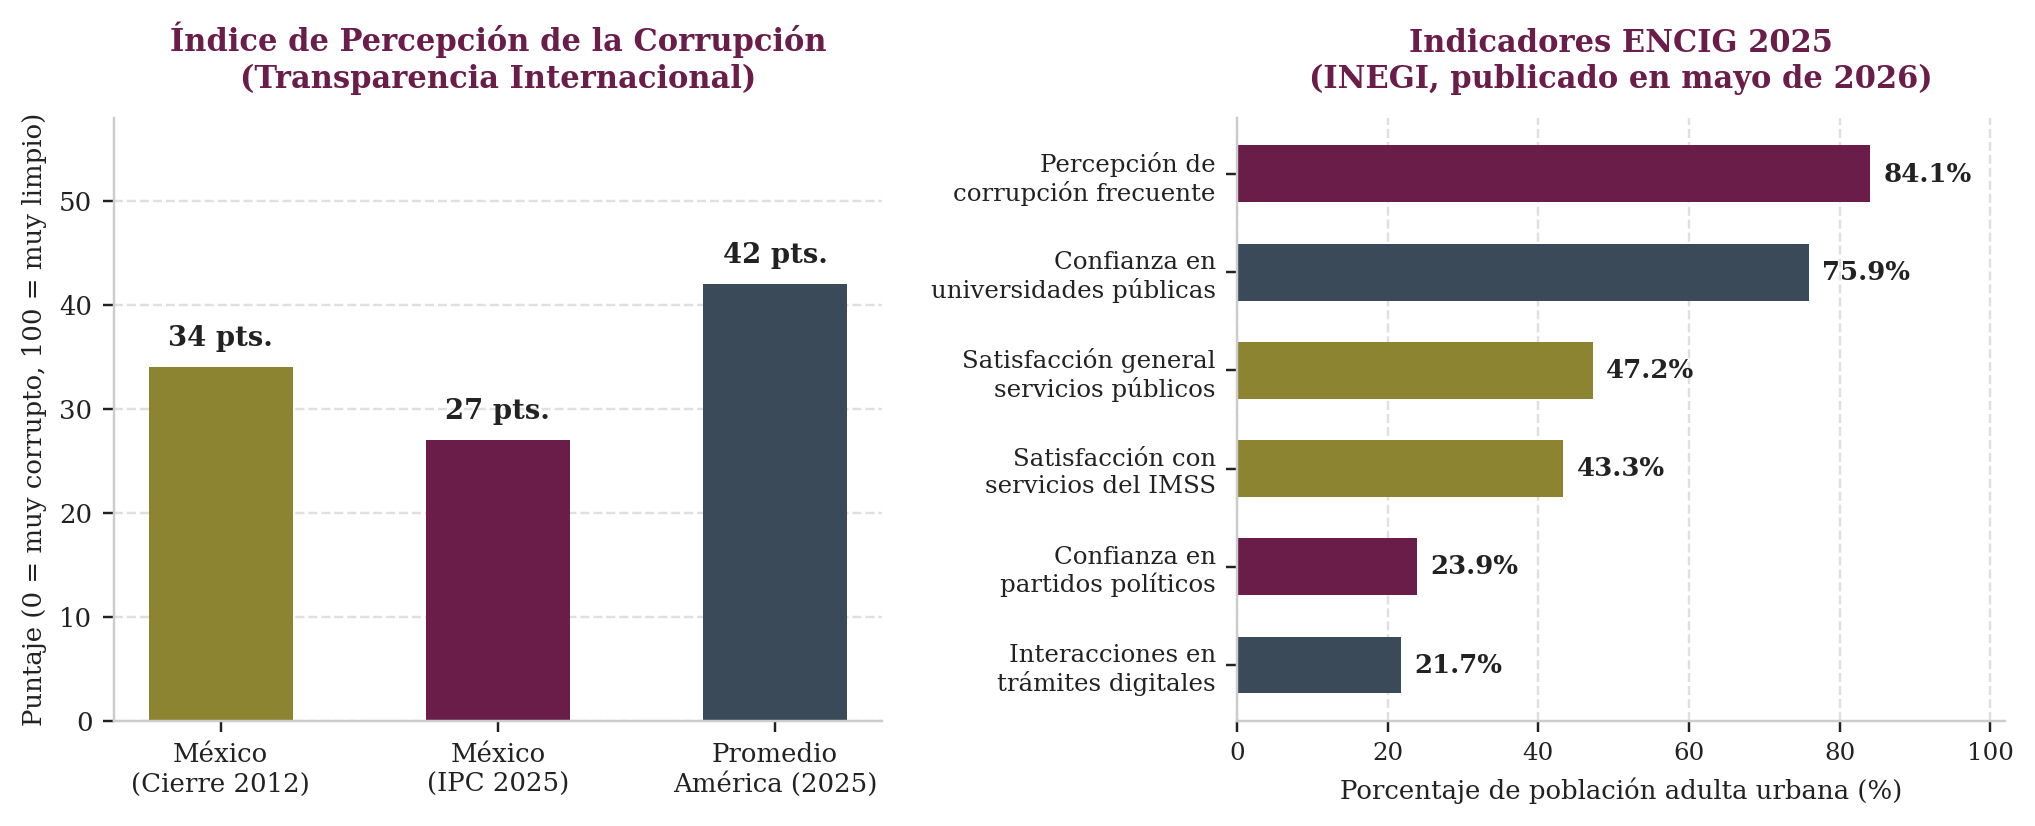
\includegraphics[width=0.9\textwidth]{img/image3.png} % Figura 1: Evolución IPC 2012 vs 2025 + ENCIG 2025
\caption{Evolución del Índice de Percepción de la Corrupción (2012 vs. 2025) e indicadores nacionales de la ENCIG 2025. Fuente: Elaboración propia con datos de Transparencia Internacional (2026) e INEGI (2026).}
\label{fig:ipc-encig}
\end{figure}

\clearpage

% Capítulo 7: Hipótesis
\chapter{Hipótesis y operacionalización}

% ═══════════════════════════════════════════════════════════════════════════════
% HIPÓTESIS - INSTITUTO ATENEO DE COLIMA
% Estudio Documental: Corrupción en México (2006-2012)
% ═══════════════════════════════════════════════════════════════════════════════

\nota{
  Este capítulo formula la hipótesis de trabajo conforme a los estándares de 
  Hernández Sampieri (2014) para estudios documentales de casos múltiples. 
  La hipótesis orienta el análisis documental sin pretender generalización 
  estadística.
}

\section{Hipótesis de trabajo u orientadora}

En congruencia con los lineamientos de Hernández Sampieri et al. (2014) para estudios cualitativos y mixtos de modelo dominante cualitativo basados en casos múltiples, en esta investigación se formuló una hipótesis de trabajo u orientadora (Hi) ---y no una hipótesis causal estadística sujeta a prueba probabilística--- con el propósito de guiar la recolección documental, la codificación categorial y la integración de metainferencias:

\textbf{Hipótesis de trabajo u orientadora (Hi):} Los episodios emblemáticos de corrupción registrados durante el sexenio de Felipe Calderón (2006--2012) no respondieron a fallas administrativas aisladas, sino a condiciones estructurales de concentración discrecional de poder sin contrapesos, planeación presupuestal deficiente en obra pública y desregulación de servicios subrogados con conflicto de interés, lo cual se asoció con efectos prolongados sobre la integridad institucional, el erario público y los derechos humanos ---observables en los casos Genaro García Luna, Refinería Bicentenario y Guardería ABC---, cuya magnitud verificable difiere con frecuencia de la jerarquía asignada por el encuadre mediático.

De la hipótesis de trabajo se derivaron tres supuestos orientadores específicos correspondientes a cada caso principal:

\begin{enumerate}
  \item \textbf{Supuesto 1 (Seguridad y captura institucional):} La concentración de mando operativo, inteligencia y presupuesto en la Secretaría de Seguridad Pública, sin contrapesos efectivos de fiscalización interna ni control bilateral, generó condiciones propicias para la captura institucional y la operación paralela de redes de cohecho criminal y desvío contractual.
  
  \item \textbf{Supuesto 2 (Megainfraestructura y finanzas públicas):} La adopción de decisiones políticas prematuras en megainfraestructura, carente de estudios técnicos vinculantes y candados presupuestales transexenales, convirtió proyectos estratégicos como la Refinería Bicentenario en pasivos fiscales prolongados sin rentabilidad social ni productiva.
  
  \item \textbf{Supuesto 3 (Subrogación y derechos humanos):} La expansión acelerada de la subrogación de servicios públicos esenciales bajo requisitos flexibilizados y vínculos de conflicto de interés diluyó la responsabilidad administrativa del Estado y elevó los riesgos sobre derechos fundamentales, como ocurrió en la Guardería ABC.
\end{enumerate}

Se estableció explícitamente que la evidencia recopilada a partir de tres casos intencionales únicamente permite valorar la congruencia empírico-documental con la hipótesis de trabajo y generar hallazgos analíticamente transferibles, sin pretender una comprobación definitiva ni una generalización estadística hacia la totalidad de la Administración Pública Federal 2006--2012 \citep{hernandez2014}.

\section{Operacionalización de categorías y variables}

\begin{table}[H]
\centering
\caption{Operacionalización de categorías, variables e indicadores documentales}
\label{tab:operacionalizacion}
\small
\begin{tabular}{@{}p{3.5cm}p{5cm}p{5cm}@{}}
\toprule
\textbf{Componente analítico} & \textbf{Categorías / variables examinadas} & \textbf{Indicadores empíricos y documentales verificados} \\
\midrule
\multirow{3}{3.5cm}{Condiciones institucionales (factores asociados)} & 
1. Concentración discrecional de poder sin contrapesos. \newline
2. Debilidad en preinversión y fiscalización de obra pública. \newline
3. Desregulación y conflicto de interés en servicios subrogados. & 
Expansión operativa y presupuestal en la SSP sin procesamiento interno; auditorías técnicas de preinversión de la ASF; tasa de crecimiento de guarderías subrogadas frente a directas en el IMSS y vínculos familiares/políticos registrados en expedientes. \\
\addlinespace
\multirow{3}{3.5cm}{Efectos documentados (resultados observables)} & 
1. Captura institucional y macrocriminalidad. \newline
2. Daño patrimonial y pasivos fiscales transexenales. \newline
3. Vulneración de derechos humanos y deterioro de la confianza pública. & 
Sentencias penales y civiles en EE. UU. y México; montos desviados, porcentajes de sobrecosto y amortización de deuda estatal; víctimas mortales y lesionadas; trayectoria del IPC (2012--2025) y tasas de la ENCIG 2025. \\
\addlinespace
Variable de contraste (encuadre mediático) & 
Diferencia entre atención mediática (framing) y daño verificable a la población. & 
Contraste entre titulares virales no acreditados o reduccionistas y hallazgos oficiales de auditorías, verificaciones sanitarias (COFEPRIS) y reportes operativos (Veracruz y Dos Bocas). \\
\bottomrule
\end{tabular}
\end{table}

\clearpage

% Capítulo 8: Metodología
\chapter{Marco metodológico}

% ═══════════════════════════════════════════════════════════════════════════════
% METODOLOGÍA - INSTITUTO ATENEO DE COLIMA
% Estudio Documental: Corrupción en México (2006-2012)
% ═══════════════════════════════════════════════════════════════════════════════

\nota{
  Este capítulo detalla el diseño metodológico DIAC (CUAL + cuan) aplicado 
  conforme a Hernández Sampieri (2014). Se enfatiza el carácter documental 
  del estudio y los criterios de rigor aplicados.
}

\section{Enfoque y diseño de investigación (DIAC: CUAL + cuan)}

La investigación se desarrolló bajo un enfoque mixto formalizado como un Diseño Anidado Concurrente de Modelo Dominante (DIAC: CUAL + cuan), no experimental, retrospectivo y de estudio de casos múltiples \citep{hernandez2014}. En este diseño, ambas ramas de evidencia se recolectaron de forma simultánea (concurrente), pero el proyecto fue guiado por un método dominante de naturaleza cualitativa-documental (CUAL), dentro del cual se anidó un componente cuantitativo secundario de alcance descriptivo (cuan).

La integración metodológica operó de la siguiente manera: la rama dominante (CUAL) reconstruyó los procesos institucionales, las cadenas de evidencia jurídica y las categorías analíticas (captura estatal, opacidad contractual, dilución regulatoria y encuadre mediático) a partir de resoluciones judiciales, auditorías oficiales y doctrina especializada; de forma simultánea, la rama anidada (cuan) sistematizó indicadores estadísticos y financieros secundarios oficiales (puntajes del IPC 2012 y 2025, tasas de prevalencia, percepción y costo directo de la ENCIG 2025, montos desviados, porcentajes de sobrecosto, deuda subnacional y crecimiento de concesiones del IMSS). Ambas bases de datos se cruzaron en la fase de análisis e interpretación para generar metainferencias con consistencia interpretativa, permitiendo dimensionar numéricamente los daños institucionales explicados por la evidencia cualitativa \citep{hernandez2014}.

\section{Elección y justificación del tipo de investigación}

El estudio tuvo un carácter documental, descriptivo y analítico-explicativo, bajo un diseño no experimental, retrospectivo y de estudio de casos múltiples:

\begin{itemize}
  \item \textbf{Documental:} Se sustentó en la revisión sistemática y triangulada de fuentes primarias oficiales (auditorías de la ASF, expedientes del DOJ, comunicados de la UIF, sentencias de la SCJN, recomendaciones de la CNDH, informes de la CIDH y series del INEGI) y literatura académica mexicana e internacional dictaminada.
  
  \item \textbf{Descriptiva:} Detalló las propiedades, los actores, las cuantías financieras, las cronologías procesales y los indicadores nacionales que caracterizaron la corrupción en México entre 2006 y 2026.
  
  \item \textbf{Analítico-explicativa (en lógica cualitativa de casos):} Indagó cómo se configuró cada caso desde el punto de vista institucional, vinculando fallas en el diseño de contrapesos, planeación y regulación con sus consecuencias patrimoniales y en derechos humanos.
  
  \item \textbf{No experimental, retrospectiva y de estudio de casos múltiples:} No se manipularon variables ni se conformaron grupos experimentales; se examinaron hechos consumados entre 2006 y 2012 ---junto con sus derivaciones judiciales y fiscales hasta noviembre de 2026--- mediante el contraste estructurado de tres casos principales.
\end{itemize}

\section{Identificación de la población / universo y delimitación temporal}

El universo documental principal se delimitó al conjunto de expedientes de presunta corrupción, irregularidades administrativas graves y contrataciones públicas auditadas o judicializadas correspondientes a la Administración Pública Federal mexicana durante el sexenio 2006--2012, considerando sus resoluciones judiciales y pasivos financieros rastreables hasta noviembre de 2026. Como marco de referencia empírica nacional para la rama cuantitativa anidada, se emplearon los universos estadísticos oficiales de la ENCIG 2025 (población adulta residente en áreas urbanas de México medida por el INEGI) y del IPC 2025 (182 países evaluados por Transparencia Internacional).

Con el propósito de preservar el rigor de la delimitación temporal y evitar cualquier desviación del recorte 2006--2012, se estableció explícitamente que los dos episodios posteriores incluidos en el subtema 3.3 ---el saqueo hospitalario en Veracruz y la Refinería Olmeca (Dos Bocas)--- no formaron parte del universo nuclear del sexenio calderonista, sino que se incorporaron estrictamente como casos de contraste contemporáneo para evaluar la variable de encuadre mediático (framing).

\section{Tipo y procedimiento para muestras (casos principales y de contraste)}

Atendiendo a la naturaleza del estudio de casos múltiples, se aplicó un muestreo no probabilístico de tipo intencional (o dirigido por criterio teórico), estrategia adecuada para profundizar en fenómenos complejos cuando el objetivo es la riqueza documental y no la estimación estadística poblacional \citep{hernandez2014}. Del inventario documentado del sexenio 2006--2012 (que abarcó también Estela de Luz, ABB/CFE, BizJet, CPS penitenciarios, Odebrecht y Oceanografía), se seleccionó una muestra principal de tres casos emblemáticos (n = 3) ---Genaro García Luna, Refinería Bicentenario y Guardería ABC--- mediante tres criterios explícitos de inclusión:

\begin{enumerate}
  \item \textbf{Diversidad tipológica:} representar tres mecanismos analíticos diferenciados de corrupción (captura del aparato de seguridad pública, deficiencias de planeación y pasivos en megainfraestructura, y desregulación con conflicto de interés en servicios públicos subrogados).
  
  \item \textbf{Rigor probatorio oficial:} contar con evidencia emitida por órganos jurisdiccionales, fiscalizadores o de derechos humanos de ámbito nacional o internacional (cortes federales y civiles de EE. UU., UIF, ASF, SCJN, CNDH y CIDH).
  
  \item \textbf{Magnitud del impacto social y patrimonial:} documentar afectaciones verificables sobre la seguridad pública, el erario federal o estatal y derechos humanos fundamentales.
\end{enumerate}

Adicionalmente, para cumplir el cuarto objetivo específico relativo al encuadre mediático, se integraron por criterio teórico dos casos de contraste contemporáneo (Veracruz y Refinería Olmeca/Dos Bocas) cuya función metodológica se circunscribió a comparar la divergencia entre narrativas virales y evidencia oficial en materia de salud e infraestructura energética.

\section{Justificación y descripción de la técnica para recolección de datos}

Se empleó la técnica de análisis documental estructurado con triangulación de fuentes. Esta elección se justificó porque los esquemas de gran corrupción, lavado transnacional y captura institucional poseen un carácter clandestino que impide medirlos adecuadamente mediante cuestionarios de opinión local; en cambio, requieren reconstruir cadenas de evidencia cotejando resoluciones judiciales, auditorías técnicas, estadísticas oficiales y literatura académica. Para sistematizar la información se diseñaron y aplicaron dos instrumentos ---cuyos formatos modelo se presentan en los Apéndices A y B---:

\begin{itemize}
  \item \textbf{Ficha de Registro Jurídico-Institucional y Hemerográfico:} Instrumento cualitativo destinado a registrar el código de expediente, periodo, dependencias involucradas, tipología delictiva o administrativa, fuentes primarias trianguladas, hechos probados, posturas de descargo y categorías codificadas (Apéndice A).
  
  \item \textbf{Matriz Comparativa de Variables, Dimensiones e Indicadores por Caso:} Instrumento mixto de integración que cruzó las categorías cualitativas (mecanismo institucional, fallas de control y encuadre mediático) con los indicadores cuantitativos anidados (presupuestos, sobrecostos, deuda, sentencias pecuniarias y número de víctimas) en cada caso (Apéndice B).
\end{itemize}

\section{Método para análisis descriptivo y cualitativo-analítico}

En estricto apego a Hernández Sampieri et al. (2014, caps. 8 y 10), se declara expresamente que, debido a que la investigación empleó un muestreo no probabilístico intencional de tres casos documentales (n = 3), NO se aplicó estadística inferencial paramétrica ni no paramétrica para estimar parámetros poblacionales ni someter hipótesis a pruebas de significancia estadística. En su lugar, el procesamiento de la información integró dos procedimientos complementarios propios de un diseño DIAC (CUAL + cuan):

\begin{enumerate}
  \item \textbf{Estadística descriptiva (rama anidada cuan):} Se utilizó exclusivamente para organizar y describir los indicadores secundarios oficiales ---frecuencias absolutas y relativas, puntajes del IPC (2012 y 2025), tasas de prevalencia por cada 100 mil habitantes, promedios de gasto por víctima de la ENCIG 2025, porcentajes de sobrecosto presupuestal, evolución numérica de guarderías del IMSS y montos fijados en sentencias civiles--- sin proyectar inferencias probabilísticas fuera de sus fuentes originales.
  
  \item \textbf{Análisis cualitativo categorial, triangulación de fuentes e inferencia analítica comparada (rama dominante CUAL):} Constituyó el núcleo analítico de la investigación. Consistió en la codificación categorial de los documentos recopilados en torno a cuatro ejes (captura estatal, planeación presupuestal, regulación/conflicto de interés y framing mediático), la triangulación entre resoluciones judiciales, auditorías de la ASF y doctrina académica, y la inferencia analítica comparada entre los tres casos principales y los dos de contraste, con el objetivo de construir metainferencias trazables y analíticamente transferibles.
\end{enumerate}

\clearpage

% Capítulo 9: Caso 1
\chapter{Captura institucional y macrocriminalidad: Genaro García Luna}

% ═══════════════════════════════════════════════════════════════════════════════
% CASO 1: CAPTURA INSTITUCIONAL Y MACROCRIMINALIDAD - INSTITUTO ATENEO DE COLIMA
% Estudio Documental: Genaro García Luna (2006-2012)
% ═══════════════════════════════════════════════════════════════════════════════

\nota{
  Este capítulo analiza la captura institucional del aparato de seguridad pública 
  mediante evidencia judicial (DOJ 2024), auditorías (ASF) y doctrina académica 
  (Astorga 2015; Vázquez Valencia 2019). La reconstrucción se basa exclusivamente 
  en fuentes públicas oficiales verificables.
}

\section{Ascenso técnico e inicio de la colusión (1989--2006)}

La reconstrucción biográfico-institucional demostró que la red de poder de García Luna no se originó en diciembre de 2006, sino que se consolidó de manera progresiva a lo largo de más de dos décadas dentro del aparato mexicano de inteligencia y seguridad. Ingeniero mecánico egresado de la Universidad Autónoma Metropolitana, ingresó en 1989 como agente en el Centro de Investigación y Seguridad Nacional (CISEN), donde se especializó en contraterrorismo y combate al secuestro y articuló vínculos estrechos con mandos políticos, policiales y militares \citep{castillog2023,expansion2019}.

En 1999 se incorporó a la recién creada Policía Federal Preventiva y en diciembre de 2000 asumió la dirección de la Policía Judicial Federal. Durante el gobierno de Vicente Fox (2001--2006), diseñó y encabezó la Agencia Federal de Investigación (AFI), proyectando una reputación internacional de modernizador policial avalada por reconocimientos de INTERPOL y agencias estadounidenses, aun frente a controversias públicas graves como el montaje televisivo del caso Florence Cassez en diciembre de 2005 \citep{astorga2007,expansion2019}. No obstante, de acuerdo con las pruebas acreditadas posteriormente ante la justicia federal de Estados Unidos, fue desde el año 2001 cuando comenzaron sus acuerdos de soborno y colusión con el Cártel de Sinaloa \citep{doj2024garcialuna,pastrana2024}. Este hallazgo coincide con lo señalado por Flores Pérez (2009), quien documentó cómo la alternancia política sin controles efectivos sobre los cuerpos de policía permitió la infiltración de redes criminales en instituciones de seguridad.

\section{Concentración sin contrapesos y doble vertiente de corrupción (2006--2012)}

Al iniciar su mandato, Felipe Calderón nombró a García Luna titular de la Secretaría de Seguridad Pública (SSP), otorgándole una concentración inédita de presupuesto, inteligencia y mando operativo en el marco de la estrategia contra el narcotráfico \citep{astorga2015}. Bajo su gestión, el estado de fuerza de la Policía Federal se expandió de alrededor de 5,000 a más de 35,000 efectivos al cierre del sexenio \citep{pastrana2024}. Dicha concentración discrecional ---en ausencia de contrapesos horizontales efectivos \citep{lopezayllon2009,zaid2019}--- se asoció con la operación simultánea de dos vertientes de gran corrupción:

\subsection{Protección criminal (cohecho y abuso de funciones)}

En el expediente 19-CR-576 (S-1) (BMC) sustanciado en la Corte Federal del Distrito Este de Nueva York, la fiscalía acreditó que el exsecretario recibió decenas de millones de dólares en sobornos en efectivo del Cártel de Sinaloa. A cambio, facilitó el tráfico de más de un millón de kilogramos de cocaína hacia Estados Unidos, filtró información de inteligencia sobre operativos en curso y dirigió acciones policiales contra organizaciones competidoras \citep{doj2024garcialuna,insightcrime2023}. Al dictar sentencia, el juez federal Brian Cogan resumió la magnitud institucional del caso al señalar que el acusado llevó una «doble vida» equiparable a la de los capos que combatía públicamente \citep{pastrana2024}. En el plano operativo interno, su colaborador cercano y exdirector de Seguridad Regional de la Policía Federal, Luis Cárdenas Palomino, fue detenido en México en 2021 por el delito de tortura y figuró en las indagatorias estadounidenses.

\subsection{Red contractual y lavado de activos (peculado y desvío de recursos)}

De forma paralela a los sobornos del narcotráfico, a partir de 2009 ---con continuidad transexenal hasta 2018 en contratos con el CISEN, la Policía Federal, el Órgano Administrativo Desconcentrado Prevención y Readaptación Social (OADPRS) y la entonces Procuraduría General de Justicia de la Ciudad de México--- García Luna articuló junto con la familia empresarial Weinberg (Mauricio Samuel y Jonathan Alexis Weinberg) una estructura corporativa offshore registrada en Panamá e Israel (Nunvav Inc., Nunvav Technologies, Nice Systems Ltd. y la consultora GLAC) \citep{mcci2023,castilloj2026}. La Unidad de Inteligencia Financiera (UIF) documentó 30 contratos públicos por más de 727 millones de dólares y 528 millones de pesos para equipamiento tecnológico y mantenimiento penitenciario, cuyos fondos fueron dispersados hacia cuentas en Barbados, Israel y México y hacia empresas factureras identificadas por el SAT \citep{uif2024,mcci2023}.

\section{Judicialización internacional, sentencias y posturas de descargo (2019--2026)}

Aunque diversas denuncias públicas y señalamientos internos se habían formulado años atrás sin traducirse en procesos penales firmes dentro de México, la ruptura judicial se produjo en el extranjero. Tras ser arrestado por agentes de la DEA en Dallas, Texas, en diciembre de 2019, Genaro García Luna fue declarado culpable de cinco cargos federales vinculados al narcotráfico y falsedad de declaraciones en febrero de 2023, y condenado el 16 de octubre de 2024 a más de 38 años de prisión, sentencia que comenzó a purgar en la penitenciaría federal de máxima seguridad ADX Florence \citep{doj2024garcialuna}.

En la vía civil patrimonial, la demanda promovida por el Estado mexicano mediante la UIF ante cortes de Florida obtuvo resoluciones condenatorias de alta cuantía: el 22 de mayo de 2025, un tribunal de Miami ordenó a García Luna y a su esposa, Linda Cristina Pereyra, resarcir aproximadamente 2,500 millones de dólares al Estado mexicano (1,740 millones correspondientes a Pereyra) \citep{uif2025,guillen2025}. Posteriormente, el 17 de noviembre de 2026, la Secretaría de Hacienda y Crédito Público notificó la obtención de una nueva sentencia civil favorable a México por más de 578 millones de dólares dentro del mismo entramado empresarial \citep{uif2026}.

En cumplimiento del criterio de confirmabilidad y balance probatorio, se registró la postura de descargo del expresidente Felipe Calderón, quien tras la sentencia de octubre de 2024 rechazó toda responsabilidad personal y declaró que durante su gestión nunca dispuso de «evidencia verificable que lo involucrara con actividades ilícitas» ni recibió alertas formales de agencias de inteligencia nacionales o estadounidenses, defendiendo la legalidad de su estrategia de seguridad \citep{infobae2024}. Sin embargo, el contraste entre las sentencias judiciales estadounidenses, la continuidad contractual hasta 2018 y la ausencia de sanción penal interna oportuna evidenció debilidades estructurales profundas en los mecanismos de supervisión horizontal y bilateral \citep{insightcrime2023,merino2024,vazquezvalencia2019}.

\clearpage

% Capítulo 10: Caso 2
\chapter{Megainfraestructura: Refinería Bicentenario}

% ═══════════════════════════════════════════════════════════════════════════════
% CASO 2: REFINERÍA BICENTENARIO - INSTITUTO ATENEO DE COLIMA
% Estudio Documental: Corrupción en México (2006-2012)
% ═══════════════════════════════════════════════════════════════════════════════

\nota{
  Este capítulo analiza los patrones de vulnerabilidad en megainfraestructura 
  del caso Refinería Bicentenario mediante evidencia de auditorías ASF (2015, 2016) 
  y doctrina de Cancino/BID (2020) y Sandoval Ballesteros (2024).
}

\section{Anuncio político, competencia estatal y endeudamiento subnacional (2008--2012)}

El 18 de marzo de 2008, durante la conmemoración de la expropiación petrolera, el Ejecutivo federal anunció la edificación de una nueva refinería con una inversión estimada superior a 9,000 millones de dólares. Para seleccionar la sede, Petróleos Mexicanos (Pemex) instrumentó un proceso competitivo entre entidades federativas ---en el que Hidalgo y Guanajuato llegaron como finalistas--- cuyo criterio decisivo se concentró en la donación estatal de un predio de 700 hectáreas con infraestructura básica de acceso.

Con el propósito de obtener la adjudicación de la sede en Tula de Allende, el gobierno del estado de Hidalgo adquirió parcelas ejidales y financió obras de conectividad mediante la contratación de deuda pública cercana a 1,500 millones de pesos (1,050 millones para la adquisición de tierras y 450 millones para infraestructura de acceso). Dicho compromiso financiero gravó las finanzas locales durante más de una década: la administración estatal liquidó por completo el adeudo con Banorte hasta el 18 de septiembre de 2025, diecisiete años después del anuncio presidencial y sin que la planta refinadora hubiera sido construida \citep{periodicohidalgo2025}.

Simultáneamente, entre 2009 y 2012, Pemex ejerció más de 9,000 millones de pesos (más de 620 millones de dólares) en estudios de ingeniería básica, limpieza, nivelación del terreno y la edificación de una barda perimetral con costo superior a 500 millones de pesos, sin consolidar el esquema financiero definitivo ni iniciar la construcción de las plantas industriales de proceso \citep{asf2015,asf2016,raziel2021}.

\section{Cancelación, fiscalización de la ASF y pasivos persistentes (2014--2025)}

En diciembre de 2014, durante la administración de Enrique Peña Nieto, Pemex canceló definitivamente la Refinería Bicentenario al argumentar la ausencia de rentabilidad económica frente a la coyuntura energética internacional \citep{montoya2014}. La fiscalización realizada por la Auditoría Superior de la Federación documentó deficiencias sustantivas en dos auditorías específicas:

\begin{itemize}
  \item \textbf{Auditoría de Inversiones Físicas 13-1-18T4M-04-0353 (DE-226)} sobre el Estudio de Preinversión \citep{asf2015}: Documentó inconsistencias técnicas y observaciones de fiscalización desde la etapa temprana de evaluación de factibilidad económica y de ingeniería del proyecto.
  
  \item \textbf{Auditoría 533-DE} sobre el terreno donado en Tula de Allende \citep{asf2016}: Verificó la condición improductiva de las 700 hectáreas donadas por Hidalgo y las omisiones en el resguardo patrimonial de la inversión ejercida.
\end{itemize}

Los costos fiscales continuaron acumulándose tras la cancelación: reportes sustentados en estados financieros auditados evidenciaron que Pemex siguió cubriendo pasivos vinculados al predio sin uso productivo, erogando 195.5 millones de pesos únicamente en el ejercicio 2020 \citep{raziel2021}. Como postura de descargo, en febrero de 2025 Felipe Calderón sostuvo que su administración cumplió la etapa inicial programada (ingeniería, preparación del terreno y barda perimetral) y atribuyó la pérdida del proyecto a la orden de cancelación emitida por su sucesor \citep{elfinanciero2025}.

\section{Panorama comparado de otros expedientes de obra y contratación del sexenio (2006--2012)}

La triangulación documental mostró que las vulnerabilidades observadas en Tula coexistieron con otros expedientes relevantes de obra pública, asociaciones público-privadas y sobornos corporativos registrados durante el mismo periodo:

\begin{table}[H]
\centering
\caption{Panorama comparado de otros expedientes de obra y contratación del sexenio (2006--2012)}
\label{tab:expedientes}
\small
\begin{tabular}{@{}p{2.5cm}p{4cm}p{6.5cm}@{}}
\toprule
\textbf{Expediente (2006--2012)} & \textbf{Tipología / mecanismo} & \textbf{Evidencia oficial y magnitud documentada} \\
\midrule
Estela de Luz & Sobreprecios y pagos improcedentes en obra pública. & La ASF (2013) acreditó un sobrecosto de 192\,\% (de \textasciitilde393--398 mdp a >1,104--1,146 mdp), 15 meses de retraso y 399.2 mdp en pagos improcedentes de acero \citep{asf2013,obrasexpansion2013}. \\
\addlinespace
Contratos penitenciarios (CPS) & APP opacas con pagos rígidos a 20--22 años. & Ocho CEFERESOS desde 2010; la ASF observó falta de fundamento legal claro e informes documentaron cláusulas de secrecía y pagos independientes de la ocupación real \citep{documenta2022,badillo2021}. \\
\addlinespace
Sobornos FCPA (ABB/CFE y BizJet) & Cohecho transnacional sancionado por autoridades de EE.\,UU. & Multas de 58.8 MDD (ABB/CFE) y 11.8 MDD (BizJet) por sobornos a mandos de Policía Federal y flota presidencial, con declaración de culpabilidad adicional en octubre de 2026 \citep{doj2013bizjet,doj2026bizjet,rodriguez2011}. \\
\addlinespace
Pemex: Odebrecht y Oceanografía & Continuidad transexenal y tráfico de influencias. & Contratos en Minatitlán y Etileno XXI (Odebrecht) y 54 contratos con Oceanografía entre 2002 y 2012, cuyas tramas se extendieron y judicializaron en sexenios posteriores \citep{fundar2022,guerrero2018}. \\
\bottomrule
\end{tabular}
\end{table}

\clearpage

% Capítulo 11: Caso 3
\chapter{Desregulación y derechos humanos: Guardería ABC}

% ═══════════════════════════════════════════════════════════════════════════════
% CASO 3: GUARDERÍA ABC - INSTITUTO ATENEO DE COLIMA
% Estudio Documental: Corrupción en México (2006-2012)
% ═══════════════════════════════════════════════════════════════════════════════

\nota{
  Este capítulo analiza la desregulación y conflicto de interés en el caso 
  Guardería ABC mediante evidencia de CNDH (2009), SCJN (2010, 2025) y 
  doctrina de Serna de la Garza (2010) y Osorno (2010).
}

\section{Retiro estatal, expansión de la subrogación y conflicto de interés (1995--2009)}

El incendio de la Guardería ABC en Hermosillo, Sonora, ocurrido el 5 de junio de 2009 ---en el que fallecieron 49 niñas y niños y más de 100 menores sufrieron lesiones graves---, evidenció los riesgos extremos advertidos por Rose-Ackerman (1999), Rezzoagli et al. (2021), Sandoval Ballesteros (2009) y Serna de la Garza (2010) en la interfaz entre el Estado regulador y los operadores privados cuando confluyen la desregulación, el conflicto de interés y la ausencia de vigilancia independiente.

El seguro de guarderías del Instituto Mexicano del Seguro Social (IMSS) surgió en 1973 como un servicio público directo financiado con cuotas obrero-patronales. A partir de 1995 se impulsó el esquema «vecinal-comunitario» de subrogación a particulares: entre 2000 y 2009, las estancias subrogadas aumentaron de 757 a 1,374 ---un crecimiento de 81.5\,\%---, mientras que las operadas directamente por el IMSS permanecieron congeladas en 142 \citep{leal2010}.

% FIGURA PENDIENTE
\begin{figure}[H]
\centering

\includegraphics[width=0.9\textwidth]{img/image2.png} % Figura 2: Expansión guarderías IMSS 2000-2009
\caption{Expansión de guarderías subrogadas frente a guarderías de operación directa del IMSS (2000--2009). Fuente: Elaboración propia con datos de Leal (2010).}
\label{fig:guarderias-imss}
\end{figure}

La concesión de la Guardería ABC fue otorgada a una sociedad civil integrada por particulares con vínculos familiares y políticos con altos funcionarios estatales y federales ---entre quienes figuraban Marcia Matilde Altagracia Gómez del Campo Tonella (prima de la entonces primera dama Margarita Zavala) y Sandra Lucía Téllez Nieves, además de socios ligados al gobierno de Sonora--- \citep{scjn2009,osorno2010}. Como documentaron la investigación periodística de Osorno (2010) y los expedientes de derechos humanos, la estancia operaba en una nave industrial adaptada con techumbre inflamable, salidas de emergencia deficientes y únicamente 14 de los 40 trabajadores reglamentarios el día del siniestro, colindando pared con pared con una bodega de archivo y vehículos de la Secretaría de Hacienda estatal \citep{leal2010,nunez2026}.

La Recomendación 49/2009 de la CNDH acreditó que el siniestro era previsible y evitable: existía un dictamen arquitectónico fechado en julio de 2005 que ya había señalado riesgos graves en el inmueble sin que el IMSS ni Protección Civil ordenaran correcciones o la suspensión del servicio \citep{cndh2009}. En concordancia con Serna de la Garza (2010) y Arellano Gault (2012), la transferencia desregulada del servicio y las redes informales de cercanía política diluyeron la responsabilidad pública y neutralizaron los controles preventivos.

\section{Resoluciones constitucionales e internacionales (2010--2026)}

La trayectoria jurídica del expediente consolidó precedentes relevantes en el sistema constitucional mexicano y en el ámbito interamericano:

\begin{itemize}
  \item \textbf{Suprema Corte de Justicia de la Nación (SCJN):} En el dictamen final de la Facultad de Investigación 1/2009 (ponente ministro Arturo Zaldívar) y posteriormente en la sentencia del Amparo Directo 14/2019, el alto tribunal acreditó la existencia de un «desorden generalizado» en el sistema nacional de guarderías y una subrogación efectuada al margen del artículo 213 de la Ley del Seguro Social, aunque en 2010 no se alcanzó mayoría para fincar responsabilidad directa a los titulares nacionales del IMSS \citep{scjn2010,scjn2025,zaldivar2010}.
  
  \item \textbf{Comisión Interamericana de Derechos Humanos (CIDH):} En julio de 2020, mediante el Informe No. 185/20, admitió la petición internacional al constatar la omisión de fiscalizaciones de oficio por parte del IMSS y la ampliación contractual pese a los peligros evidentes de la bodega contigua \citep{cidh2020}.
  
  \item \textbf{Declaratoria de imprescriptibilidad penal (2026):} El 19 de junio de 2026, el Pleno de la SCJN declaró imprescriptible la acción penal en el caso Guardería ABC, determinando que el paso del tiempo no extingue el derecho a la justicia ni a la reparación integral ante violaciones graves a los derechos de la niñez \citep{nunez2026}.
\end{itemize}

\section{Casos de contraste contemporáneo: daño real en derechos humanos frente a encuadre mediático (framing)}

Con el fin de responder la cuarta pregunta de investigación sin alterar la delimitación nuclear 2006--2012, se examinaron dos casos de contraste contemporáneo que permitieron contrastar el criterio de afectación verificable a derechos humanos \citep{cidh2019,acnudh} frente a las distorsiones del encuadre mediático \citep{solamorales2019}:

\subsection{Contraste 1 --- Sector salud en Veracruz}

En enero de 2017 se viralizó la acusación de que durante la gubernatura de Javier Duarte se había aplicado agua destilada a niños con cáncer. Tras veinte visitas de inspección sanitaria, la Secretaría de Salud federal y la COFEPRIS informaron oficialmente que no se encontró evidencia de medicamentos falsos ni de agua destilada suministrada a pacientes oncológicos \citep{cofepris2017}. No obstante, la narrativa viral eclipsó parcialmente un saqueo masivo plenamente comprobado: la propia COFEPRIS aseguró 46,984 pruebas rápidas de VIH caducas y sin registro y 16.8 toneladas de medicamentos caducos, mientras auditorías e investigaciones documentaron 2,933 millones de pesos desviados en obra hospitalaria (183 obras inconclusas y 12 hospitales abandonados), más de 3,617 millones de pesos transferidos a empresas fantasma y 276.6 millones adicionales en factureras ---hechos que derivaron en nuevas imputaciones de la FGR en diciembre de 2025--- \citep{connectas,animalpolitico,santiago2025,angel2025}.

\subsection{Contraste 2 --- Megainfraestructura energética (Dos Bocas)}

De modo comparable al símbolo reduccionista de «la barda» en la Refinería Bicentenario de Tula, el debate público sobre la Refinería Olmeca (Dos Bocas) tendió a polarizarse en consignas sobre si la planta «no refina un solo litro». Los reportes técnicos oficiales mostraron una realidad más matizada pero financieramente crítica: el costo se elevó de 8,000 millones de dólares proyectados a más de 21,000 millones al cierre de 2024 (\textasciitilde2.6 veces el presupuesto original) y, aunque la producción alcanzó 212,000--263,000 barriles diarios hacia finales de 2025 (frente a su capacidad nominal de 340,000), descendió a 141,000 barriles diarios en junio de 2026 tras un incendio en la planta de coque y una falla eléctrica \citep{alegria2026,martinezescamilla2026,celaya2026}. Reducir estos proyectos a eslóganes partidistas desplazó la fiscalización rigurosa sobre adjudicaciones, sobrecostos y costo de oportunidad fiscal.

\section{Ejes de corrupción en México jerarquizados por alcance poblacional}

Al jerarquizar las modalidades de corrupción documentadas en México conforme al criterio objetivo de número de afectados y vulneración de derechos fundamentales ---al margen de afinidades partidistas---, emergieron cinco ejes de impacto estructural:

\begin{table}[H]
\centering
\caption{Ejes de corrupción en México jerarquizados por alcance poblacional y derechos vulnerados}
\label{tab:ejes_corrupcion}
\small
\begin{tabular}{@{}p{3.5cm}p{4cm}p{5.5cm}@{}}
\toprule
\textbf{Eje de corrupción} & \textbf{Casos / evidencia emblemática} & \textbf{Magnitud verificable del daño y población afectada} \\
\midrule
Captura de seguridad pública y macrocriminalidad & Genaro García Luna (SSP, 2006--2012) y colusión local con crimen organizado. & Afectación sobre millones de habitantes por violencia, narcotráfico y extorsión. Condena penal de >38 años (2024) y civiles por \textasciitilde2,500 MDD (2025) y >578 MDD (2026). \\
\addlinespace
Desfalco a programas sociales y abasto alimentario & Segalmex (2019--2024) y La Estafa Maestra (2012--2018). & Irregularidades en Segalmex por >15,000--15,300 mdp destinados a pequeños productores y abasto rural; desvíos en La Estafa Maestra por >7,000 mdp en programas sociales \citep{perez2024,mccitablero}. \\
\addlinespace
Desvíos y deterioro del sector salud & Saqueo hospitalario estatal (Veracruz) e irregularidades en transferencias federales. & Impacto directo en millones de usuarios sin seguro privado; en noviembre de 2026 la ASF aún señaló 285.8 mdp por aclarar y 553.3 mdp reintegrados en salud estatal \citep{ramos2026}; IMSS con 43.3\,\% de satisfacción \citep{inegi2026}. \\
\addlinespace
Desregulación con conflicto de interés letal & Subrogación irregular en la Guardería ABC (2009). & 49 niñas y niños fallecidos y más de 100 lesionados graves; «desorden generalizado» acreditado por la SCJN e imprescriptibilidad penal decretada en junio de 2026. \\
\addlinespace
Corrupción cotidiana («mordida» en trámites) & Medición nacional ENCIG 2025 (INEGI, publ. mayo 2026). & Impuesto regresivo directo: afectó a 15.6\,\% de quienes gestionaron trámites y extrajo \$17,707.4 millones de pesos anuales (\$3,865 pesos promedio por víctima). \\
\bottomrule
\end{tabular}
\end{table}

\clearpage

% Capítulo 12: Conclusiones
\chapter{Conclusiones}

% ═══════════════════════════════════════════════════════════════════════════════
% CONCLUSIONES - INSTITUTO ATENEO DE COLIMA
% Estudio Documental: Corrupción en México (2006-2012)
% ═══════════════════════════════════════════════════════════════════════════════

\nota{
  Este capítulo sintetiza las metainferencias obtenidas mediante análisis 
  documental DIAC (CUAL + cuan) y contrasta hallazgos con literatura académica 
  (Casar y Cejudo 2024; Merino 2024; Sandoval Ballesteros 2024).
}

\section{Discusión, criterios de rigor y limitaciones del estudio}

La integración concurrente entre la evidencia documental dominante (CUAL) y las series estadísticas secundarias anidadas (cuan) permitió construir metainferencias consistentes con la literatura especializada \citep{hernandez2014}. En primer término, se observó plena convergencia entre la trayectoria descendente de México en el IPC (de 34 puntos en 2012 a 27 en 2025), el repunte del costo real de la corrupción cotidiana en la ENCIG 2025 (\$17,707.4 millones de pesos) y la evidencia cualitativa de los tres casos principales: la persistencia del fenómeno no obedece a la carencia de leyes, sino a la captura de controles horizontales, la discrecionalidad contractual y la impunidad transexenal descritas por Casar y Cejudo (2024), Merino (2024) y Sandoval Ballesteros (2024). En segundo lugar, las metainferencias mostraron que el encuadre mediático (framing) opera como un factor distorsionador de la rendición de cuentas cuando privilegia consignas virales imprecisas por encima de daños auditados y violaciones masivas a derechos humanos.

Para garantizar la calidad científica del reporte bajo un diseño DIAC de predominio cualitativo, se aplicaron cuatro criterios de rigor metodológico establecidos por Hernández Sampieri et al. (2014, cap. 14):

\begin{enumerate}
  \item \textbf{Credibilidad:} Se fortaleció mediante la triangulación sistemática de tres tipos de fuentes independientes ---resoluciones judiciales (DOJ, cortes de Florida, SCJN, CIDH), informes de fiscalización y derechos humanos (ASF, CNDH, COFEPRIS) y literatura académica mexicana e internacional arbitrada---, logrando corroboración estructural y adecuación referencial en cada caso.
  
  \item \textbf{Dependencia:} Se aseguró mediante la trazabilidad explícita de cada expediente (números de auditoría, expedientes judiciales, fechas exactas de emisión y enlaces verificables), criterios transparentes de inclusión muestral y el uso de instrumentos estandarizados de registro y cruce comparativo (Apéndices A y B), estableciendo cadenas de evidencia susceptibles de auditoría externa.
  
  \item \textbf{Confirmabilidad:} Para minimizar sesgos ideológicos o partidistas, se incorporaron expresamente las posturas de descargo del expresidente Felipe Calderón \citep{infobae2024,elfinanciero2025}, se documentó la continuidad transexenal de diversos entramados (contratos de García Luna hasta 2018, Odebrecht, Oceanografía y cancelación de Tula en 2014) y se integraron casos de contraste correspondientes a gobiernos de distinto signo político (Veracruz y Dos Bocas).
  
  \item \textbf{Transferencia analítica:} Se precisó que los hallazgos no buscan generalizarse estadísticamente a toda la Administración Pública Federal 2006--2012, sino ofrecer patrones institucionales analíticamente transferibles ---concentración de mando sin contrapesos, megainfraestructura sin candados transexenales y subrogación desregulada--- útiles para analizar otros periodos y niveles de gobierno.
\end{enumerate}

Asimismo, se reconocieron tres limitaciones metodológicas centrales que delimitan el alcance del estudio: (1) la dependencia exclusiva de fuentes documentales secundarias y archivos públicos, sin acceso a expedientes reservados ni entrevistas directas con actores judiciales o administrativos; (2) la vigencia de procedimientos aún en curso o en etapa de ejecución al cierre de noviembre de 2026 ---tales como el cobro efectivo de las sentencias civiles en Florida contra García Luna y su red empresarial, y el curso de acciones penales tras la declaratoria de imprescriptibilidad de la SCJN en el caso Guardería ABC---; y (3) la imposibilidad de realizar inferencias estadísticas hacia el universo completo de contrataciones y dependencias del sexenio 2006--2012 debido al carácter no probabilístico e intencional de la muestra (n = 3).

\section{Síntesis conclusiva y respuestas a las preguntas de investigación}

En conjunto, los tres casos principales aportaron evidencia documental congruente con la hipótesis de trabajo, con un alcance analíticamente transferible y no estadísticamente generalizable a toda la Administración Pública Federal 2006--2012. A partir de las metainferencias obtenidas, se dio respuesta puntual a las cinco preguntas de investigación:

\begin{enumerate}
  \item \textbf{Efectos verificables sobre el erario, la legitimidad y los derechos humanos:} La evidencia teórica y empírica examinada demostró que la corrupción ---desde prácticas cotidianas hasta esquemas sistémicos y de captura estatal--- produce efectos verificables y acumulativos sobre el erario (desvíos, sobrecostos y pagos indebidos que operan como impuesto regresivo), sobre la legitimidad democrática (deterioro sostenido de la confianza institucional y de la satisfacción con servicios públicos) y sobre el ejercicio de los derechos humanos fundamentales (vida, salud, seguridad y acceso equitativo a bienes públicos) \citep{cidh2019,inegi2026,monsivais2020,rios2021,roseackerman1999}.
  
  \item \textbf{Nivel y evolución empírica en México (2012--2026):} Los indicadores oficiales acreditaron la persistencia y el agravamiento de la corrupción en México más allá de un solo periodo gubernamental: la calificación nacional en el IPC descendió de 34 puntos al término de 2012 a 27 puntos en el IPC 2025, mientras que la ENCIG 2025 registró una percepción de frecuencia de 84.1\,\%, una prevalencia de 15.6\,\% en trámites y un costo directo de 17,707.4 millones de pesos anuales \citep{inegi2026,transparencia2026}.
  
  \item \textbf{Mecanismos institucionales y efectos de los tres casos principales:} En los tres expedientes del sexenio 2006--2012 se identificaron mecanismos estructurales convergentes: en el caso Genaro García Luna, la concentración sin contrapesos en la SSP se asoció con la captura de funciones de seguridad y desvíos contractuales sancionados en tribunales estadounidenses entre 2024 y 2026; en la Refinería Bicentenario, la ausencia de preinversión vinculante y candados transexenales dejó más de 9,000 millones de pesos federales sin planta productiva y una deuda estatal de 1,500 millones liquidada por Hidalgo hasta septiembre de 2025; y en la Guardería ABC, la expansión de la subrogación desregulada (81.5\,\% entre 2000 y 2009) junto con conflictos de interés y omisiones de inspección derivó en la muerte de 49 menores, cuya búsqueda de justicia alcanzó en junio de 2026 la declaratoria de imprescriptibilidad penal de la SCJN.
  
  \item \textbf{Brecha entre daño verificable y encuadre mediático:} El contraste con los episodios contemporáneos de Veracruz y Dos Bocas evidenció que la agenda mediática (framing) con frecuencia desplaza el escrutinio sobre daños masivos acreditados ---como 12 hospitales abandonados, 16.8 toneladas de medicamentos caducos o sobrecostos de 2.6 veces lo presupuestado--- hacia consignas virales imprecisas o polarizadas, debilitando la exigencia ciudadana de rendición de cuentas basada en pruebas.
  
  \item \textbf{Controles institucionales para reducir la brecha de implementación:} Con base en la literatura institucional y organizacional analizada \citep{arellanogault2012,casar2024,lopezayllon2009,merino2024,ocde2017,peschard2017}, contener la corrupción exige cerrar la brecha entre la ley y la sanción efectiva mediante cinco medidas concretas: garantizar la autonomía real de los órganos fiscalizadores y de procuración de justicia; reducir la discrecionalidad mediante la digitalización integral de trámites (apenas en 21.7\,\% en 2025); establecer candados técnicos vinculantes y transparencia abierta en megaproyectos transexenales; restituir la supervisión pública independiente y libre de conflictos de interés sobre servicios concesionados; y fortalecer la evaluación basada en indicadores verificables.
\end{enumerate}

En última instancia, observar la corrupción con la cabeza fría obliga a mirar más allá de las cifras presupuestales y los discursos coyunturales. Así como ningún proyecto duradero prospera cuando se improvisa y se abandonan los planes rigurosos, ningún país logra superar la impunidad si tolera que las reglas se doblen según conveniencias de grupo. Detrás de cada expediente documentado en estas páginas permaneció una lección difícil pero insoslayable: cuando se debilita la integridad de las instituciones, lo que realmente queda expuesto son la vida, la salud, la seguridad y el porvenir de las familias mexicanas. Reconocer con honestidad esos fallos constituye el primer paso indispensable para exigir controles que funcionen, sostener la persistencia en la rendición de cuentas y evitar que la historia vuelva a repetirse.

\clearpage

% ═══════════════════════════════════════════════════════════════════════════════
% REFERENCIAS BIBLIOGRÁFICAS
% ═══════════════════════════════════════════════════════════════════════════════

\nocite{*}
\bibliographystyle{apalike}
\bibliography{referencias-corrupcion-calderon}

\clearpage

% ═══════════════════════════════════════════════════════════════════════════════
% APÉNDICES
% ═══════════════════════════════════════════════════════════════════════════════

\appendix

\chapter{Ficha de Registro Jurídico-Institucional y Hemerográfico}

% ═══════════════════════════════════════════════════════════════════════════════
% APÉNDICE A: FICHA DE REGISTRO JURÍDICO-INSTITUCIONAL - INSTITUTO ATENEO DE COLIMA
% Estudio Documental: Corrupción en México (2006-2012)
% ═══════════════════════════════════════════════════════════════════════════════

\nota{
  Este apéndice presenta el instrumento documental utilizado para registrar 
  sistemáticamente la evidencia oficial de cada caso. La ficha garantiza 
  trazabilidad y reproducibilidad del análisis documental.
}

\section{Ficha de Registro Jurídico-Institucional y Hemerográfico}

\begin{table}[H]
\centering
\caption{Formato de Ficha de Registro (Apéndice A)}
\label{tab:ficha_registro}
\small
\begin{tabular}{@{}p{4cm}p{10cm}@{}}
\toprule
\textbf{Campo de registro} & \textbf{Descripción operativa / criterio de llenado} \\
\midrule
Código de ficha y fecha & Ej.: F-01 / Fecha de consulta y última verificación (DD/MM/AAAA). \\
\addlinespace
Caso y clasificación muestral & Nombre del caso $|$ [$\Box$] Caso principal (2006--2012) [$\Box$] Caso de contraste contemporáneo (framing). \\
\addlinespace
Periodo de hechos y seguimiento & Años de origen (ej. 2006--2012) y corte de resoluciones judiciales/fiscales (hasta nov. 2026). \\
\addlinespace
Dependencias y actores & Instituciones federales/estatales, contratistas, operadores privados y autoridades jurisdiccionales. \\
\addlinespace
Tipología de irregularidad & [$\Box$] Cohecho [$\Box$] Peculado [$\Box$] Captura estatal [$\Box$] Conflicto de interés [$\Box$] Mala planeación [$\Box$] Negligencia regulatoria. \\
\addlinespace
Fuentes primarias oficiales & Sentencias judiciales (expediente y corte), auditorías ASF (clave), recomendaciones CNDH/CIDH. \\
\addlinespace
Respaldo académico y verificación & Libros arbitrados, artículos científicos y periodismo de verificación. \\
\addlinespace
Posturas de descargo y continuidad & Declaraciones oficiales de defensa y vínculos del esquema con administraciones previas o posteriores. \\
\addlinespace
Categorías codificadas y trazabilidad & Códigos temáticos asignados, estatus procesal y vínculo entre evidencia CUAL y datos cuan. \\
\bottomrule
\end{tabular}
\end{table}

\section{Ejemplo de Ficha Completada: Caso Genaro García Luna}

\begin{table}[H]
\centering
\caption{Ficha de Registro: Caso Genaro García Luna (F-01)}
\label{tab:ficha_ejemplo}
\small
\begin{tabular}{@{}p{4cm}p{10cm}@{}}
\toprule
\textbf{Campo} & \textbf{Contenido} \\
\midrule
Código y fecha & F-01 / 15/11/2026 \\
\addlinespace
Caso & Genaro García Luna (SSP 2006--2012) \\
\addlinespace
Clasificación & [$\times$] Caso principal (2006--2012) [$\Box$] Contraste \\
\addlinespace
Periodo & 2001--2018 (colusión desde 2001; contratos hasta 2018) \\
\addlinespace
Dependencias & SSP, AFI, CISEN, OADPRS, PGJCDMX \\
\addlinespace
Tipología & [$\times$] Cohecho [$\times$] Peculado [$\times$] Captura estatal [$\Box$] Conflicto de interés [$\Box$] Mala planeación [$\Box$] Negligencia \\
\addlinespace
Fuentes primarias & DOJ 19-CR-576 (2024); UIF (2024, 2025, 2026); ASF (contratos tecnológicos) \\
\addlinespace
Respaldo académico & Astorga (2015); Vázquez Valencia (2019); Flores Pérez (2009) \\
\addlinespace
Posturas descargo & Calderón (Infobae 2024): «Nunca tuve evidencia verificable» \\
\addlinespace
Categorías & Captura institucional; macrocriminalidad; red offshore \\
\bottomrule
\end{tabular}
\end{table}

\clearpage

\chapter{Matriz Comparativa de Variables, Dimensiones e Indicadores}

% ═══════════════════════════════════════════════════════════════════════════════
% APÉNDICE B: MATRIZ COMPARATIVA - INSTITUTO ATENEO DE COLIMA
% Estudio Documental: Corrupción en México (2006-2012)
% ═══════════════════════════════════════════════════════════════════════════════

\nota{
  Este apéndice presenta la matriz comparativa utilizada para integrar 
  evidencia cualitativa (mecanismos institucionales) con indicadores 
  cuantitativos anidados (montos, víctimas, sentencias). La matriz 
  permite generar metainferencias trazables por caso.
}

\section{Matriz Comparativa de Variables, Dimensiones e Indicadores por Caso}

\begin{landscape}
\begin{table}[H]
\centering
\caption{Matriz Comparativa por Caso (Apéndice B)}
\label{tab:matriz_comparativa}
\tiny
\begin{tabular}{@{}p{2cm}p{2.5cm}p{3.5cm}p{4cm}p{6.5cm}@{}}
\toprule
\textbf{Caso y tipo} & \textbf{Dimensión analítica / factor asociado} & \textbf{Mecanismo institucional (CUAL)} & \textbf{Indicadores cuantitativos (cuan)} & \textbf{Fuentes trianguladas (APA 7)} \\
\midrule
Caso 1 (Principal) \newline Genaro García Luna & Concentración de mando, presupuesto e inteligencia en SSP sin contrapesos. & Captura estatal y macrocriminalidad: cohecho con Cártel de Sinaloa + red offshore Weinberg. & PF: 5,000 a >35,000; 30 contratos (>727 MDD y 528 mdp); prisión >38 años (2024); civiles \textasciitilde2,500 MDD (2025) y >578 MDD (2026). & DOJ (2024, exp. 19-CR-576); UIF (2024, 2025, 2026); Astorga (2015); Vázquez Valencia (2019); Infobae (2024). \\
\addlinespace
Caso 2 (Principal) \newline Refinería Bicentenario & Anuncio político prematuro, preinversión débil y sin candados transexenales. & Opacidad y mala planeación en megainfraestructura con transferencia de pasivos. & Proyección >9,000 MDD; gasto Pemex >9,000 mdp; barda >500 mdp; deuda Hidalgo \textasciitilde1,500 mdp liquidada sep. 2025; 195.5 mdp en 2020. & ASF (2015, 2016); Cancino (2020); Sandoval Ballesteros (2024); El Financiero (2025). \\
\addlinespace
Caso 3 (Principal) \newline Guardería ABC & Desregulación de estancias IMSS, conflicto de interés y omisión de inspecciones. & Subrogación desregulada con dilución de la responsabilidad administrativa estatal. & Subrogadas: 757 a 1,374 (+81.5\,\%) vs. 142 directas; 14 de 40 empleados; 49 fallecidos y >100 lesionados graves. & CNDH (2009); SCJN (2009, 2010, 2025); Núñez Esquer (2026); CIDH (2020); Serna de la Garza (2010); Osorno (2010). \\
\addlinespace
Contraste 1 \newline Sector Salud Veracruz & Saqueo presupuestal y empresas fantasma; encuadre viral impreciso. & Contraste entre rumor mediático («agua destilada») y desvío hospitalario acreditado. & 0 evidencia agua destilada (COFEPRIS); 46,984 pruebas VIH y 16.8 t fármacos caducos; 2,933 mdp obra; >3,617 mdp fantasma. & Secretaría de Salud / COFEPRIS (2017); Connectas (s.\,f.); Animal Político (s.\,f.); Santiago y Morales (2025); Ángel (2025); Sola-Morales y Zurbano-Berenguer (2019). \\
\addlinespace
Contraste 2 \newline Refinería Olmeca / Dos Bocas & Sobrecostos en megainfraestructura y polarización en eslóganes partidistas. & Contraste entre consigna viral («no refina») y desempeño técnico-financiero real. & Costo: 8,000 a >21,000 MDD (\textasciitilde2.6x); producción 212--263 mil bd (fin 2025) con caída a 141 mil bd (jun. 2026). & Alegría (2026); Martínez Escamilla (2026); El Universal / Celaya (2026); Cancino (2020); Reyes Heroles (2003). \\
\bottomrule
\end{tabular}
\end{table}
\end{landscape}

\clearpage

\end{document}

% ═══════════════════════════════════════════════════════════════════════════════
% FIN DEL DOCUMENTO
% ═══════════════════════════════════════════════════════════════════════════════
